% Options for packages loaded elsewhere
\PassOptionsToPackage{unicode}{hyperref}
\PassOptionsToPackage{hyphens}{url}
%
\documentclass[
]{article}
\usepackage{amsmath,amssymb}
\usepackage{lmodern}
\usepackage{ifxetex,ifluatex}
\ifnum 0\ifxetex 1\fi\ifluatex 1\fi=0 % if pdftex
  \usepackage[T1]{fontenc}
  \usepackage[utf8]{inputenc}
  \usepackage{textcomp} % provide euro and other symbols
\else % if luatex or xetex
  \usepackage{unicode-math}
  \defaultfontfeatures{Scale=MatchLowercase}
  \defaultfontfeatures[\rmfamily]{Ligatures=TeX,Scale=1}
\fi
% Use upquote if available, for straight quotes in verbatim environments
\IfFileExists{upquote.sty}{\usepackage{upquote}}{}
\IfFileExists{microtype.sty}{% use microtype if available
  \usepackage[]{microtype}
  \UseMicrotypeSet[protrusion]{basicmath} % disable protrusion for tt fonts
}{}
\makeatletter
\@ifundefined{KOMAClassName}{% if non-KOMA class
  \IfFileExists{parskip.sty}{%
    \usepackage{parskip}
  }{% else
    \setlength{\parindent}{0pt}
    \setlength{\parskip}{6pt plus 2pt minus 1pt}}
}{% if KOMA class
  \KOMAoptions{parskip=half}}
\makeatother
\usepackage{xcolor}
\IfFileExists{xurl.sty}{\usepackage{xurl}}{} % add URL line breaks if available
\IfFileExists{bookmark.sty}{\usepackage{bookmark}}{\usepackage{hyperref}}
\hypersetup{
  pdftitle={Permutation Tests},
  pdfauthor={Livio Finos},
  hidelinks,
  pdfcreator={LaTeX via pandoc}}
\urlstyle{same} % disable monospaced font for URLs
\usepackage[margin=1in]{geometry}
\usepackage{color}
\usepackage{fancyvrb}
\newcommand{\VerbBar}{|}
\newcommand{\VERB}{\Verb[commandchars=\\\{\}]}
\DefineVerbatimEnvironment{Highlighting}{Verbatim}{commandchars=\\\{\}}
% Add ',fontsize=\small' for more characters per line
\usepackage{framed}
\definecolor{shadecolor}{RGB}{248,248,248}
\newenvironment{Shaded}{\begin{snugshade}}{\end{snugshade}}
\newcommand{\AlertTok}[1]{\textcolor[rgb]{0.94,0.16,0.16}{#1}}
\newcommand{\AnnotationTok}[1]{\textcolor[rgb]{0.56,0.35,0.01}{\textbf{\textit{#1}}}}
\newcommand{\AttributeTok}[1]{\textcolor[rgb]{0.77,0.63,0.00}{#1}}
\newcommand{\BaseNTok}[1]{\textcolor[rgb]{0.00,0.00,0.81}{#1}}
\newcommand{\BuiltInTok}[1]{#1}
\newcommand{\CharTok}[1]{\textcolor[rgb]{0.31,0.60,0.02}{#1}}
\newcommand{\CommentTok}[1]{\textcolor[rgb]{0.56,0.35,0.01}{\textit{#1}}}
\newcommand{\CommentVarTok}[1]{\textcolor[rgb]{0.56,0.35,0.01}{\textbf{\textit{#1}}}}
\newcommand{\ConstantTok}[1]{\textcolor[rgb]{0.00,0.00,0.00}{#1}}
\newcommand{\ControlFlowTok}[1]{\textcolor[rgb]{0.13,0.29,0.53}{\textbf{#1}}}
\newcommand{\DataTypeTok}[1]{\textcolor[rgb]{0.13,0.29,0.53}{#1}}
\newcommand{\DecValTok}[1]{\textcolor[rgb]{0.00,0.00,0.81}{#1}}
\newcommand{\DocumentationTok}[1]{\textcolor[rgb]{0.56,0.35,0.01}{\textbf{\textit{#1}}}}
\newcommand{\ErrorTok}[1]{\textcolor[rgb]{0.64,0.00,0.00}{\textbf{#1}}}
\newcommand{\ExtensionTok}[1]{#1}
\newcommand{\FloatTok}[1]{\textcolor[rgb]{0.00,0.00,0.81}{#1}}
\newcommand{\FunctionTok}[1]{\textcolor[rgb]{0.00,0.00,0.00}{#1}}
\newcommand{\ImportTok}[1]{#1}
\newcommand{\InformationTok}[1]{\textcolor[rgb]{0.56,0.35,0.01}{\textbf{\textit{#1}}}}
\newcommand{\KeywordTok}[1]{\textcolor[rgb]{0.13,0.29,0.53}{\textbf{#1}}}
\newcommand{\NormalTok}[1]{#1}
\newcommand{\OperatorTok}[1]{\textcolor[rgb]{0.81,0.36,0.00}{\textbf{#1}}}
\newcommand{\OtherTok}[1]{\textcolor[rgb]{0.56,0.35,0.01}{#1}}
\newcommand{\PreprocessorTok}[1]{\textcolor[rgb]{0.56,0.35,0.01}{\textit{#1}}}
\newcommand{\RegionMarkerTok}[1]{#1}
\newcommand{\SpecialCharTok}[1]{\textcolor[rgb]{0.00,0.00,0.00}{#1}}
\newcommand{\SpecialStringTok}[1]{\textcolor[rgb]{0.31,0.60,0.02}{#1}}
\newcommand{\StringTok}[1]{\textcolor[rgb]{0.31,0.60,0.02}{#1}}
\newcommand{\VariableTok}[1]{\textcolor[rgb]{0.00,0.00,0.00}{#1}}
\newcommand{\VerbatimStringTok}[1]{\textcolor[rgb]{0.31,0.60,0.02}{#1}}
\newcommand{\WarningTok}[1]{\textcolor[rgb]{0.56,0.35,0.01}{\textbf{\textit{#1}}}}
\usepackage{graphicx}
\makeatletter
\def\maxwidth{\ifdim\Gin@nat@width>\linewidth\linewidth\else\Gin@nat@width\fi}
\def\maxheight{\ifdim\Gin@nat@height>\textheight\textheight\else\Gin@nat@height\fi}
\makeatother
% Scale images if necessary, so that they will not overflow the page
% margins by default, and it is still possible to overwrite the defaults
% using explicit options in \includegraphics[width, height, ...]{}
\setkeys{Gin}{width=\maxwidth,height=\maxheight,keepaspectratio}
% Set default figure placement to htbp
\makeatletter
\def\fps@figure{htbp}
\makeatother
\setlength{\emergencystretch}{3em} % prevent overfull lines
\providecommand{\tightlist}{%
  \setlength{\itemsep}{0pt}\setlength{\parskip}{0pt}}
\setcounter{secnumdepth}{5}
\ifluatex
  \usepackage{selnolig}  % disable illegal ligatures
\fi

\title{Permutation Tests}
\author{Livio Finos}
\date{University of Padova}

\begin{document}
\maketitle

{
\setcounter{tocdepth}{2}
\tableofcontents
}
\hypertarget{introduction}{%
\section{Introduction}\label{introduction}}

\hypertarget{introduction-1}{%
\subsection{Introduction}\label{introduction-1}}

\begin{itemize}
\tightlist
\item
  Well established nonparametric approach to \textbf{inference}: Fisher,
  1935; Pitman, 1937; Pitman, 1938.\\
\item
  (In general) it requires less assumptions about the data generating
  process than the parametric counterpart.\\
\item
  Very good inferential properties, typically:

  \begin{itemize}
  \tightlist
  \item
    exactness (i.e.~exact control of the type I error)
  \item
    asymptotically optimality and convergence to the parametric
    counterpart when it does exist.
  \end{itemize}
\end{itemize}

\begin{itemize}
\tightlist
\item
  Fisher exact test is a prototypical example, but
\item
  the general approach has restricted applicability without the support
  of a computer.
\end{itemize}

\hypertarget{renewed-interest-toward-permutation-testing}{%
\subsection{Renewed interest toward permutation
testing}\label{renewed-interest-toward-permutation-testing}}

\begin{itemize}
\tightlist
\item
  A milestone: Westfall and Young (1993). Resampling-Based Multiple
  Testing: Examples and Methods for p-value Adjustment. Wiley.
\item
  Many actives areas of research adopt these methods in their daily
  statistical analysis (e.g.~genetics and neuroscience: Nichols and
  Holmes (2002); Pantazis et al.~(2009); Winkler et al.~(2014)).\\
\item
  Permutation approach:

  \begin{itemize}
  \tightlist
  \item
    Ideal for \textbf{randomized experimental design}\\
  \item
    deals with very complex models, without formal definition of the
    data generating process.
  \end{itemize}
\end{itemize}

\hypertarget{the-package-flip}{%
\subsection{\texorpdfstring{The package
\texttt{flip}}{The package flip}}\label{the-package-flip}}

It is on CRAN and on github (\url{https://github.com/livioivil/flip})

To install the github version type (in R):

\begin{Shaded}
\begin{Highlighting}[]
\FunctionTok{library}\NormalTok{(devtools)}
\FunctionTok{install\_github}\NormalTok{(}\StringTok{\textquotesingle{}livioivil/flip\textquotesingle{}}\NormalTok{)}
\end{Highlighting}
\end{Shaded}

\textbf{Before we start}

\begin{Shaded}
\begin{Highlighting}[]
\CommentTok{\#clean the memory}
\FunctionTok{rm}\NormalTok{ (}\AttributeTok{list=}\FunctionTok{ls}\NormalTok{ ())}


\CommentTok{\# We customize the output of our graphs a little bit}
\NormalTok{par.old}\OtherTok{=}\FunctionTok{par}\NormalTok{ ()}
\FunctionTok{par}\NormalTok{ (}\AttributeTok{cex.main=}\FloatTok{1.5}\NormalTok{, }\AttributeTok{lwd=}\DecValTok{2}\NormalTok{, }\AttributeTok{col=}\StringTok{"darkgrey"}\NormalTok{, }\AttributeTok{pch=}\DecValTok{20}\NormalTok{, }\AttributeTok{cex=}\DecValTok{3}\NormalTok{)}
\CommentTok{\# par (par.old)}
\FunctionTok{palette}\NormalTok{ (}\FunctionTok{c}\NormalTok{ (}\StringTok{"\#FF0000"}\NormalTok{, }\StringTok{"\#00A08A"}\NormalTok{, }\StringTok{"\#FFCC00"}\NormalTok{, }\StringTok{"\#445577"}\NormalTok{, }\StringTok{"\#45abff"}\NormalTok{))}

\CommentTok{\# customize the output of knitr}
\NormalTok{knitr }\SpecialCharTok{::}\NormalTok{ opts\_chunk}\SpecialCharTok{$}\FunctionTok{set}\NormalTok{ (}\AttributeTok{fig.align=}\StringTok{"center"}\NormalTok{)}\CommentTok{\#, fig.width=6, fig.height=6)}
\end{Highlighting}
\end{Shaded}

\hypertarget{the-age-vs-reaction-time-dataset}{%
\subsection{The Age vs Reaction Time
Dataset}\label{the-age-vs-reaction-time-dataset}}

The reaction time of these subjects was tested by having them grab a
meter stick after it was released by the tester. The number of
centimeters that the meter stick dropped before being caught is a direct
measure of the person's response time.

The values of \texttt{Age} are in years. The \texttt{Gender} is coded as
\texttt{F} for female and \texttt{M} for male. The values of
\texttt{Reaction.Time} are in centimeters.

(data are fictitious)

To read the data

\begin{Shaded}
\begin{Highlighting}[]
\FunctionTok{data}\NormalTok{(reaction,}\AttributeTok{package =} \StringTok{"flip"}\NormalTok{)}
\CommentTok{\# or download it from: https://github.com/livioivil/flip/tree/master/data}
\CommentTok{\# str (reaction)}
\end{Highlighting}
\end{Shaded}

We plot the data

\begin{Shaded}
\begin{Highlighting}[]
\FunctionTok{plot}\NormalTok{(}\AttributeTok{x=}\NormalTok{reaction}\SpecialCharTok{$}\NormalTok{Age,}\AttributeTok{y=}\NormalTok{reaction}\SpecialCharTok{$}\NormalTok{Reaction.Time,}\AttributeTok{pch=}\DecValTok{20}\NormalTok{,}\AttributeTok{col=}\DecValTok{2}\NormalTok{,}\AttributeTok{cex=}\DecValTok{2}\NormalTok{)}
\end{Highlighting}
\end{Shaded}

\begin{center}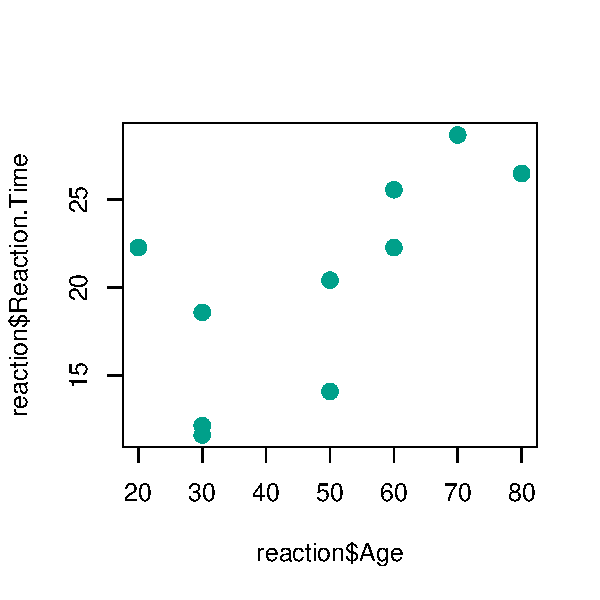
\includegraphics{perm_files/figure-latex/unnamed-chunk-4-1} \end{center}

\hypertarget{measuring-the-dependence-between-two-variables}{%
\subsection{Measuring the dependence between two
variables}\label{measuring-the-dependence-between-two-variables}}

we define:

\begin{itemize}
\tightlist
\item
  \(X=Age\)\\
\item
  \(Y=Reaction.Time\)
\end{itemize}

We review some famous index to measure the (linear) dependence among two
variables

\hypertarget{covariance-and-variance}{%
\subsubsection{Covariance and Variance}\label{covariance-and-variance}}

\textbf{Covariance} between \(X\) and \(Y\):

\(\sigma_{xy}=\frac{\sum_{i=1} ^ n (x_i- \bar{x}) (y_i- \bar{y} )}{n}\)

\begin{itemize}
\tightlist
\item
  values between \(- \infty\) and \(\infty\)\\
\item
  \(\sigma_{xy} \approx 0\): there is no dependency between \(X\) and
  \(Y\)\\
\item
  \(\sigma_{xy} >> (<<) 0\): there is a strong positive (negative)
  dependency between \(X\) and \(Y\)
\end{itemize}

\textbf{Variance} of \(X\)

\(\sigma_{xx}=\sigma_{x} ^ 2= \frac{\sum_{i=1} ^ n (x_i- \bar{x}) ^ 2}{n}\)

\textbf{Standard Deviation} of \(X\):

\(\sigma_{xx}=\sqrt{\sigma_{xx}}=\sigma_{x}\)

\hypertarget{correlation}{%
\subsubsection{Correlation}\label{correlation}}

With the Covariance it is difficult to understand when the relationship
between \(X\) and \(Y\) is strong/weak. We note that

\(- \sigma_{x} \sigma_{y} \leq \sigma_{xy} \leq \sigma_{x} \sigma_{y}\)
is quivalent to
\(-1 \leq \frac{\sigma_{xy}}{\sigma_{x} \sigma_{y}} \leq 1\)

\textbf{Correlation} between \(X\) and \(Y\):

\(\rho_{xy}=\frac{\sigma{xy}}{\sigma_{x} \sigma_{y}} = \frac{\sum_{i=1} ^ n (x_i- \bar{x}) (y_i- \bar{y})}{\sqrt{\sum_{i=1} ^ n (x_i- \bar{ x}) ^ 2} \sqrt{\sum_{i=1} ^ n (y_i- \bar{y}) ^ 2}}\)

\begin{itemize}
\tightlist
\item
  values between \(-1\) and \(1\)
\item
  \(\rho_{xy} \approx 0\): there is no dependency between \(X\) and
  \(Y\)
\item
  \(\rho_{xy} \approx 1 (-1)\): there is a strong positive (negative)
  dependency between \(X\) and \(Y\)
\end{itemize}

\hypertarget{linear-trend-the-least-squares-method}{%
\subsubsection{Linear Trend, the least squares
method}\label{linear-trend-the-least-squares-method}}

We describe the relationship between\\
\texttt{Reaction.Time} and \texttt{Age} with a straight line.

\(E(Reaction.Time) \approx \beta_0 + \beta_1 Age\)\\
\(E(Y)=\beta_0 + \beta_1X\)

Let's draw a line `in the middle' of the data.

The \textbf{least-squares estimator}

We look for the one that passes more `in the middle', the one that
minimizes the sum of the squares of the residues:

\(\hat{\beta}_0\) and \(\hat{\beta}_1\) such that\\
\(\sum_{i=1} ^ n (y_i - (\hat{\beta}_0 + \hat{\beta}_1x_i )) ^ 2\) is
minimum.

Estimates:

\begin{itemize}
\tightlist
\item
  Angular coefficient:
  \(\hat{\beta}_1=\frac{\sigma_{xy}}{\sigma_{xx}}=\rho_{xy}\frac{\sigma_{y}}{\sigma_{x}}=\frac{\sum_{i=1}^n(x_i- \bar{x})(y_i-\bar{y})}{\sum_{i=1}^n (x_i-\bar{x})^2}=\)
  0.2064719\\
\item
  Intercept: \(\hat{\beta}_0=\bar{y}-\hat{\beta}_1\bar{x}=\) 10.3013483
\item
  Response (estimated \(y\)):
  \(\hat{y}_i=\hat{\beta}_0 + \hat{\beta}_1x_i\)
\item
  Residuals (from the estimated response):
  \(y_i - (\hat{\beta}_0 + \hat{\beta}_1 x_i)=y_i- \hat{y}_i\)
\end{itemize}

and therefore the least squares are the sum of the squared residuals:
\(\sum_{i=1} ^ n (y_i- \hat{\beta}_0 + \hat{\beta}_1x_i) ^ 2=\sum_{i=1} ^ n (y_i- \hat{y}_i ) ^ 2\)

A graphical representation:

\begin{Shaded}
\begin{Highlighting}[]
\NormalTok{model}\OtherTok{=}\FunctionTok{lm}\NormalTok{(Reaction.Time}\SpecialCharTok{\textasciitilde{}}\NormalTok{Age,}\AttributeTok{data=}\NormalTok{reaction)}
\FunctionTok{coefficients}\NormalTok{(model)}
\end{Highlighting}
\end{Shaded}

\begin{verbatim}
## (Intercept)         Age 
##  10.3013483   0.2064719
\end{verbatim}

\begin{Shaded}
\begin{Highlighting}[]
\FunctionTok{plot}\NormalTok{(reaction}\SpecialCharTok{$}\NormalTok{Age,reaction}\SpecialCharTok{$}\NormalTok{Reaction.Time,}\AttributeTok{pch=}\DecValTok{20}\NormalTok{,}\AttributeTok{col=}\DecValTok{2}\NormalTok{,}\AttributeTok{cex=}\DecValTok{1}\NormalTok{)}
\NormalTok{coeff}\OtherTok{=}\FunctionTok{round}\NormalTok{(}\FunctionTok{coefficients}\NormalTok{(model),}\DecValTok{1}\NormalTok{)}
\FunctionTok{title}\NormalTok{(}\FunctionTok{paste}\NormalTok{(}\StringTok{"Y="}\NormalTok{,coeff[}\DecValTok{1}\NormalTok{],}\StringTok{"+"}\NormalTok{,coeff[}\DecValTok{2}\NormalTok{],}\StringTok{"*X"}\NormalTok{))}
\FunctionTok{abline}\NormalTok{(model,}\AttributeTok{col=}\DecValTok{1}\NormalTok{)}
\end{Highlighting}
\end{Shaded}

\begin{center}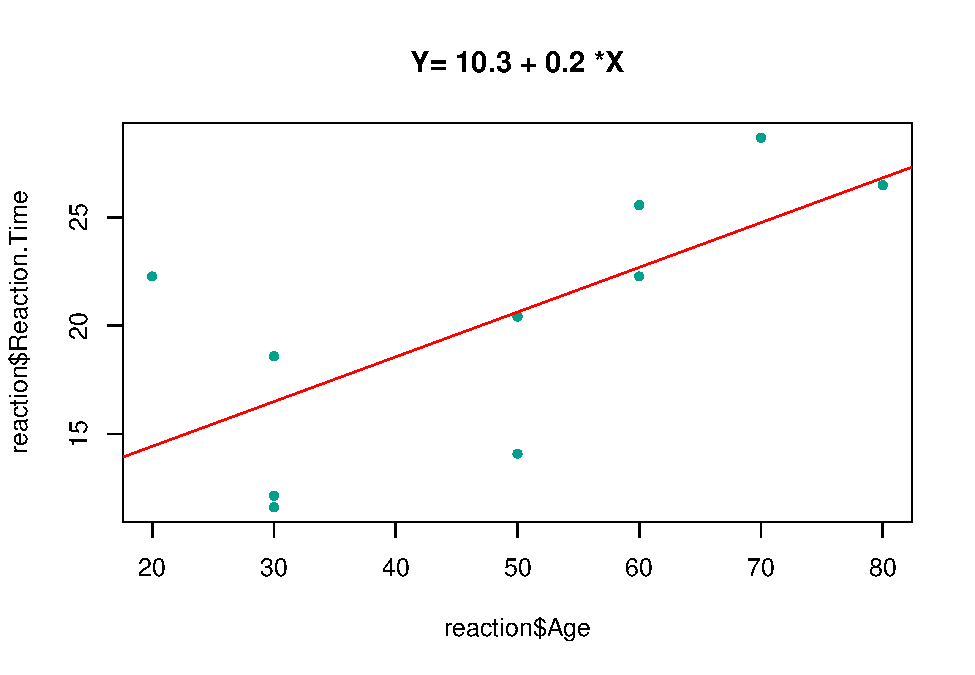
\includegraphics{perm_files/figure-latex/unnamed-chunk-7-1} \end{center}

\hypertarget{permutation-approach-to-hypothesis-testing}{%
\section{Permutation approach to Hypothesis
Testing}\label{permutation-approach-to-hypothesis-testing}}

\hypertarget{some-remarks}{%
\subsubsection{Some remarks}\label{some-remarks}}

Let's note that all the measures above does not make any assumptions on
the random process that generate them.

Let now assume that \(Y\) - and possibly \(X\) - is generated by a
random variable.

Further minimal assumptions will be specified later.

The question: \textbf{Is there a relationship between \(Y\) and \(X\)}?

We estimated \(\hat{\beta}_1=\) 0.2064719

But the \textbf{true value} \(\beta_1\) is really different from 0
(i.e.~no relationship)?\\
Otherwise, is the difference from 0 due to the random sampling?

\begin{itemize}
\item
  \textbf{Null Hypothesis} \(H_0: \ \beta_1=0\) (the \textbf{true}
  \(\beta_1\), not its estimate \(\hat{\beta}_1\)!). There is no
  relationship between \(X\) and \(Y\).
\item
  \textbf{Alternative Hypothesis }\(H_1: \ \beta_1 >0\) The relationship
  is positive.
\end{itemize}

Other possible specifications of \(H_1: \ \beta_1< 0\) and, more
commonly, \(H_1: \ \beta_1 \neq 0\).

\hypertarget{permutation-tests---in-a-nutshell}{%
\subsection{Permutation tests - in a
nutshell}\label{permutation-tests---in-a-nutshell}}

As a toy example, let use a sub-set of the data:

\begin{verbatim}
##   Age Gender Reaction.Time
## 2  50      F         20.42
## 3  30      M         11.62
## 4  60      F         22.27
\end{verbatim}

\begin{center}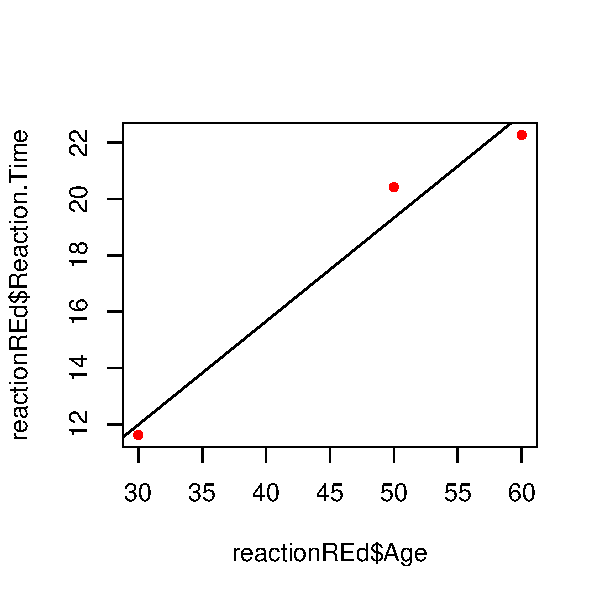
\includegraphics{perm_files/figure-latex/unnamed-chunk-8-1} \end{center}

\begin{itemize}
\tightlist
\item
  \emph{If \(H_0\)} is true: there is no linear relationship between
  \(X\) and \(Y\)
\item
  Therefore, the trend observed on the data is due to chance.
\item
  Any other match of \(x_i\) and \(y_i\) was equally likely to occur
\item
  I can generate the datasets of other hypothetical experiments by
  exchanging the order of the observations in \(Y\).
\item
  How many equally likely datasets could I get with\(X\) and
  \(Y\)observed? \(3 * 2 * 1=3!=6\) possible datasets.
\end{itemize}

Remark: Here we only assume that \(y\) is a random variable. The only
assumption here is the exchangeability of the observations: the joint
density \(f(y_1,\ldots,y_n)\) does not change when the ordering of
\(y_1,\ldots,y_n\) is changed.

\hypertarget{all-potential-datasets}{%
\subsubsection{All potential datasets}\label{all-potential-datasets}}

\begin{center}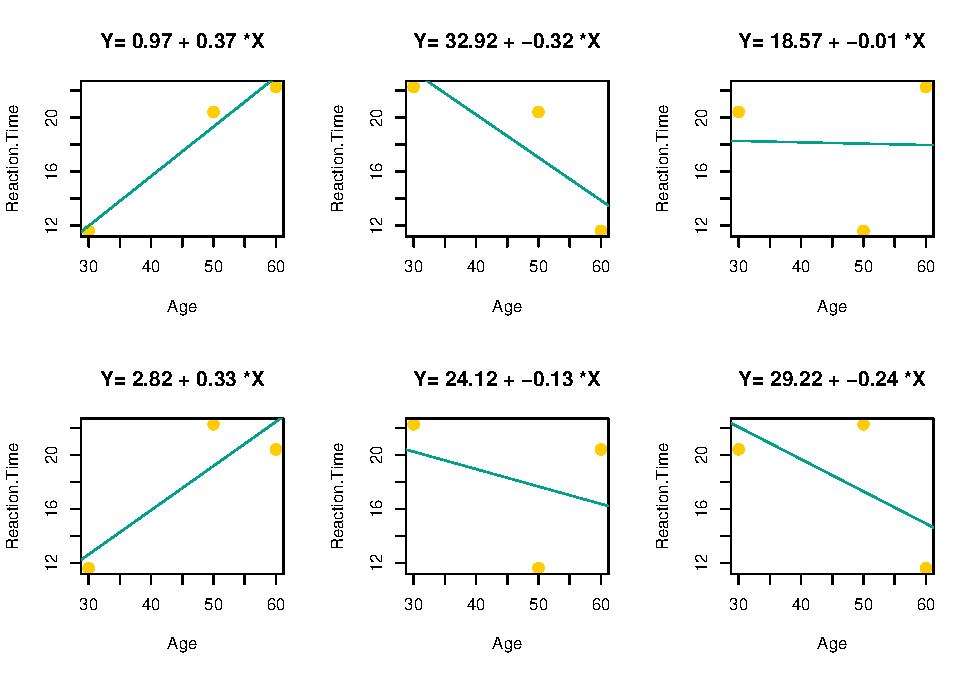
\includegraphics{perm_files/figure-latex/unnamed-chunk-9-1} \end{center}

\hypertarget{in-our-data-set}{%
\paragraph{In our data set}\label{in-our-data-set}}

We apply the same principle to the complete dataset\ldots{}

How many permutations of the vector \(y_1,\ldots,y_n\) are possible?
\(n!=10!=3628800\).

big, perhaps not too big \ldots{} but what happen with, for example,
\(n=20\)? We got \(20!=2.432902e+18\). This is too big, definitely!

We calculate a smaller (but sufficiently large) \(B\) of random
permutations.

here some example

\textbf{\texttt{Age} vs a permutations of \texttt{Reaction.Time}}

\begin{center}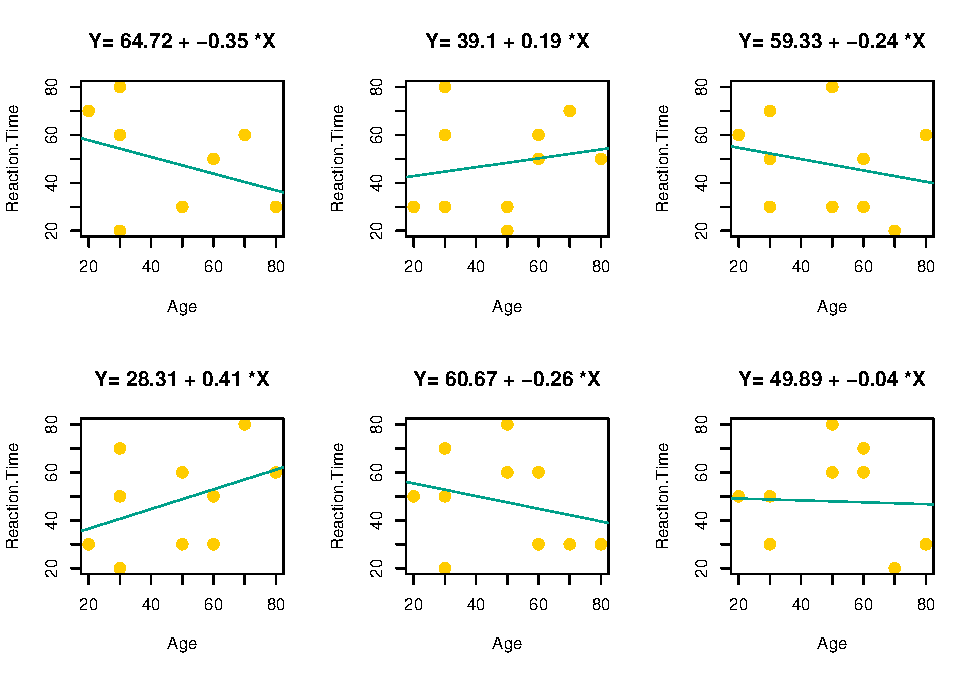
\includegraphics{perm_files/figure-latex/unnamed-chunk-10-1} \end{center}

We repeat \ensuremath{10^{4}} times and we look at the histogram of the
\(\hat{\beta}_1\)

\begin{Shaded}
\begin{Highlighting}[]
\CommentTok{\# beta\_1 estimated on the observed data:}
\NormalTok{beta1}\OtherTok{=}\FunctionTok{coefficients}\NormalTok{(}\FunctionTok{lm}\NormalTok{(Reaction.Time}\SpecialCharTok{\textasciitilde{}}\NormalTok{Age,}\AttributeTok{data=}\NormalTok{reaction))[}\DecValTok{2}\NormalTok{]}

\CommentTok{\# function that permutes the y values and calculates the coeff beta\_1}
\NormalTok{my.beta.perm }\OtherTok{\textless{}{-}} \ControlFlowTok{function}\NormalTok{(Y,X)\{}
\NormalTok{  model}\OtherTok{=}\FunctionTok{lm}\NormalTok{(}\FunctionTok{sample}\NormalTok{(Y)}\SpecialCharTok{\textasciitilde{}}\NormalTok{X)}
  \FunctionTok{coefficients}\NormalTok{(model)[}\DecValTok{2}\NormalTok{]}
\NormalTok{\}}

\CommentTok{\#replicate it B{-}1 times}
\NormalTok{beta.perm}\OtherTok{=} \FunctionTok{replicate}\NormalTok{(B,}\FunctionTok{my.beta.perm}\NormalTok{(reaction}\SpecialCharTok{$}\NormalTok{Reaction.Time, reaction}\SpecialCharTok{$}\NormalTok{Age ))}
\end{Highlighting}
\end{Shaded}

\begin{center}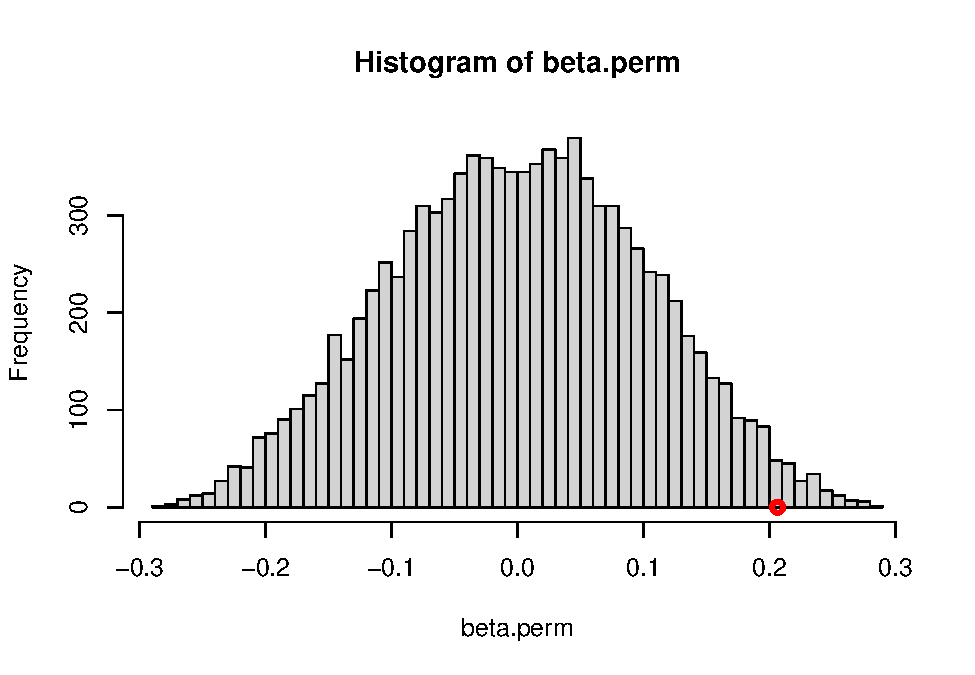
\includegraphics{perm_files/figure-latex/unnamed-chunk-12-1} \end{center}

\hypertarget{how-likely-was-hatbeta_1-obs}{%
\subsubsection{\texorpdfstring{How likely WAS
\(\hat{\beta}_1 ^{obs}\)?}{How likely WAS \textbackslash hat\{\textbackslash beta\}\_1 \^{}\{obs\}?}}\label{how-likely-was-hatbeta_1-obs}}

(before the experiment!)

How likely was it to get a \(\leq \hat{\beta}_1 ^{obs}\) value among the
many possible values of \(\hat{\beta}_1 ^{*b}\) (obtained by permuting
data)?

Remarks:

\begin{itemize}
\tightlist
\item
  \(\hat{\beta}_1 ^{* b}< \hat{\beta}_1 ^{obs}\) (closer to 0): less
  evidence against \(H_1\) than \(\hat{\beta}_1 ^{obs}\)
\item
  \(\hat{\beta}_1 ^{* b} \geq \hat{\beta}_1 ^{obs}\): equal or more
  evidence towards \(H_1\) than \(\hat{\beta}_1 ^{obs}\)
\end{itemize}

\hypertarget{calculation-of-the-p-value}{%
\subsubsection{Calculation of the
p-value}\label{calculation-of-the-p-value}}

Over B=\ensuremath{10^{4}} permutations we got 9831 times a
\(\hat{\beta}_1 ^{* b} \leq \hat{\beta}_1 ^{obs}\).

The p-value (significance) is
\(p=\frac{\# (\hat{\beta}_1 ^{* b} \geq \hat{\beta}_1 ^{obs})}{B} =\)
0.0171

(\(\hat{\beta}_1 ^{obs}\) counts as a random permutation)

\hypertarget{interpretation}{%
\subsubsection{Interpretation}\label{interpretation}}

The probability of \(p=P (\hat{\beta}_1 ^ * \geq \hat{\beta}_1=\) 0.206
\(| H_0)\) is equal to \(p =\) 0.0171, i.e.~very small.\\
So, it was unlikely to get a value like this \textbf{IF \(H_0\) is
true}.

Neyman-Pearson's approach has made common the use of a significance
threshold for example \(\alpha=.05\) (or \(=. 01\)). When
\(p \leq \alpha\) rejects the hypothesis that there is no relationship
between X and Y (\(H_0\)). If so, we are inclined to think that \(H_1\)
is true (there is a positive relationship).

\begin{itemize}
\tightlist
\item
  Type I error: False Positive\\
  the true hypo is \(H_0\) (null correlation), BUT we accept \(H_1\)
  (correlation is positive)
\item
  Type II error: False Negative\\
  the true hypo is \(H_1\) (positive correlation), BUT we do not reject
  \(H_0\) (null correlation)
\end{itemize}

\hypertarget{to-sum-up}{%
\subsection{To sum up}\label{to-sum-up}}

\textbf{p-value}: proportion of experiments providing equal or more
evidence against \(H_0\) with respect to observed data.

To compute it, we need the \textbf{Orbit \(\mathcal{O}\)} and a
\textbf{Test statistic} (\(T:\ \mathbb{R}^n\to\mathbb{R}\)) quantifies
the evidence against \(H_0\)

\begin{itemize}
\tightlist
\item
  higher values provide more evidence against \(H_0\)
\item
  compute a test statistic for each element of the Orbit
  \(\mathcal{O}\), this induces an ordering on \(\mathcal{O}\).
\end{itemize}

In our example: \(T=\hat\beta_1=\hat\sigma_{xy}/\hat\sigma_{yy}\) is the
(estimated) slope.\\
Higher the slope, higher the evidence for \(H_1\).

\textbf{Type I error control}

We want to guarantee not to get false relationships (a few false
positives), better to be conservative. To make this, we want to bound
the probability to make a false discovery:

\(P (p-value \leq \alpha | H_0) \leq \alpha\)

We built a machinery that in the long run (many replicates of the
experiment) finds false correlations with probability \(\alpha\)
(e.g.~\(0.05=5\%\)).

\hypertarget{we-make-it-in-flip}{%
\subsubsection{We make it in flip}\label{we-make-it-in-flip}}

\begin{Shaded}
\begin{Highlighting}[]
\FunctionTok{library}\NormalTok{(flip)}

\NormalTok{(}\AttributeTok{res=}\FunctionTok{flip}\NormalTok{(Reaction.Time}\SpecialCharTok{\textasciitilde{}}\NormalTok{Age,}\AttributeTok{data=}\NormalTok{reaction,}\AttributeTok{tail=}\DecValTok{1}\NormalTok{))}
\end{Highlighting}
\end{Shaded}

\begin{verbatim}
## 
##               Test  Stat tail p-value
## Reaction.Time    t 2.633    >  0.0260
\end{verbatim}

\begin{Shaded}
\begin{Highlighting}[]
\DocumentationTok{\#\# compare also with}
\CommentTok{\# flip(Reaction.Time\textasciitilde{}Age,data=reaction,tail=1,statTest = "cor")}
\CommentTok{\# flip(Reaction.Time\textasciitilde{}Age,data=reaction,tail=1,statTest = "coeff")}
\end{Highlighting}
\end{Shaded}

\begin{Shaded}
\begin{Highlighting}[]
\FunctionTok{plot}\NormalTok{(res)}
\end{Highlighting}
\end{Shaded}

\begin{center}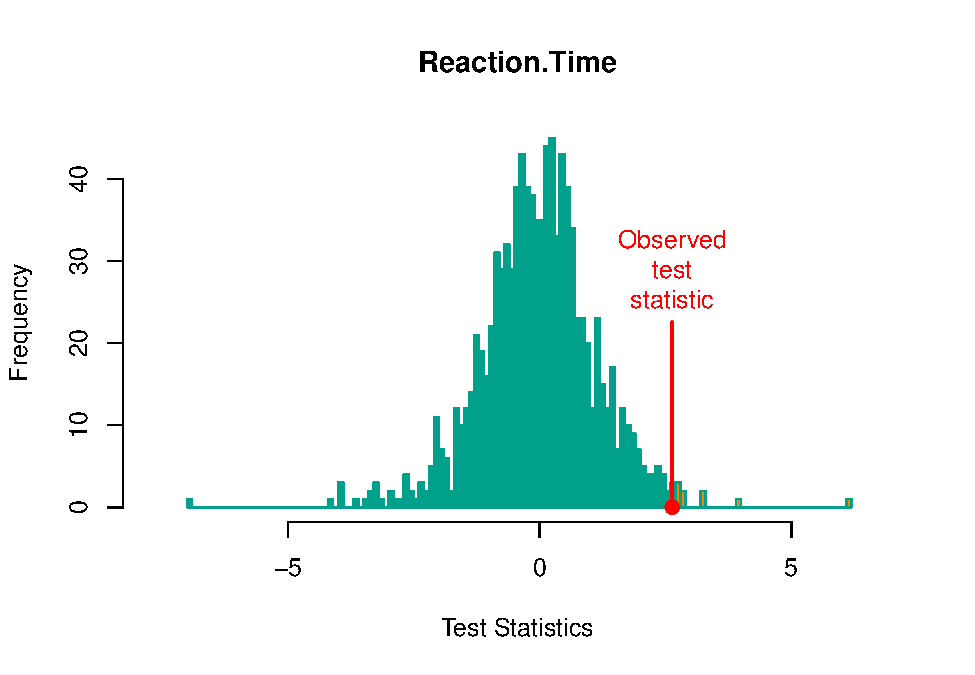
\includegraphics{perm_files/figure-latex/unnamed-chunk-14-1} \end{center}

\textbf{Type I error control}

We want to guarantee not to get false relationships (a few false
positives), better to be conservative. To make this, we want to bound
the probability to make a false discovery:

\(P (p-value \leq \alpha | H_0) \leq \alpha\)

We built a machinery that in the long run (many replicates of the
experiment) finds false correlations with probability \(\alpha\)
(e.g.~\(0.05=5\%\)).

\hypertarget{composite-alternatives-bilateral}{%
\subsubsection{Composite alternatives
(bilateral)}\label{composite-alternatives-bilateral}}

The hypothesis \(H_1: \ \beta_1 >0\) (the relation is positive) must be
justified with a priori knowledge.

More frequently, the Alternative hypothesis is appropriate:
\(H_1: \ \beta_1 \neq 0\) (there is a relationship, I do not assume the
direction)

I consider anomalous coefficients estimated as very small but also very
large (`far from 0'). The p-value is

\(p=\frac{\#(|\hat{\beta}_1^{*b} | \geq|\hat{\beta}_1^{obs}|)}{B}=\)
0.0347

(remark: the observed test stat is included among the permuted one)

In \texttt{flip}:

\begin{Shaded}
\begin{Highlighting}[]
\FunctionTok{library}\NormalTok{(flip)}
\NormalTok{(}\AttributeTok{res=}\FunctionTok{flip}\NormalTok{(Reaction.Time}\SpecialCharTok{\textasciitilde{}}\NormalTok{Age,}\AttributeTok{data=}\NormalTok{reaction,}\AttributeTok{tail=}\DecValTok{0}\NormalTok{,}\AttributeTok{perms=}\DecValTok{10000}\NormalTok{))}
\end{Highlighting}
\end{Shaded}

\begin{verbatim}
## 
##               Test  Stat tail p-value
## Reaction.Time    t 2.633   ><  0.0362
\end{verbatim}

\begin{Shaded}
\begin{Highlighting}[]
\FunctionTok{plot}\NormalTok{(res)}
\end{Highlighting}
\end{Shaded}

\begin{center}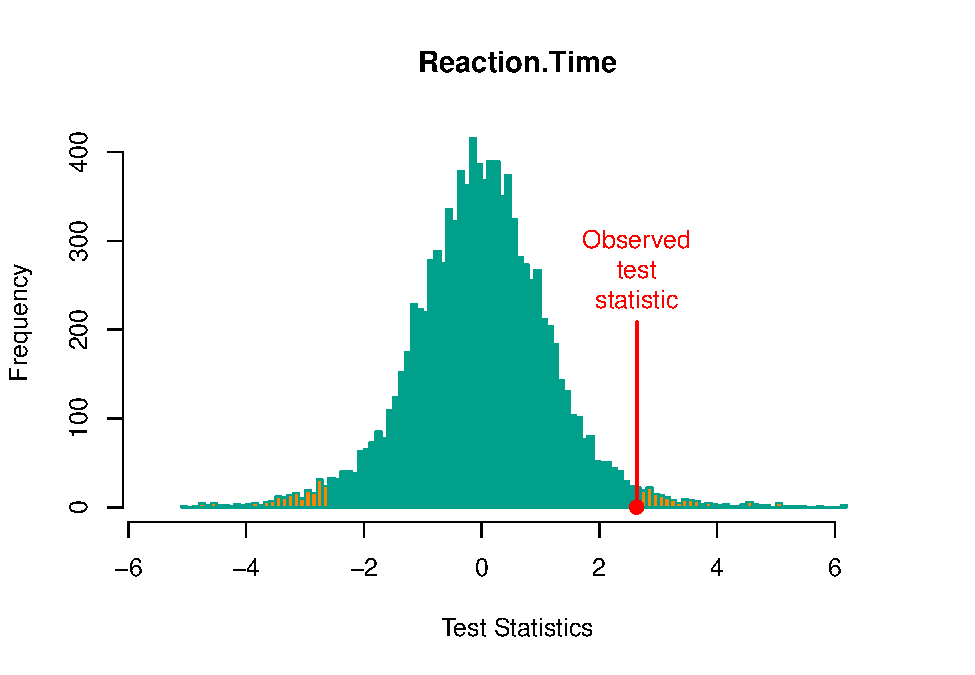
\includegraphics{perm_files/figure-latex/unnamed-chunk-16-1} \end{center}

\hypertarget{a-more-formal-approach}{%
\subsection{A more formal approach}\label{a-more-formal-approach}}

(see also Pesarin, 2001; Hemerik \& Goeman, 2017)

Let \(Y\) be data taking values in a sample space \(\mathcal{Y}\). Let
\(\Pi\) be a finite set of transformations
\(\pi : \mathcal{Y} \rightarrow \mathcal{Y}\), such that \(\Pi\) is a
\textbf{group} with respect to the operation of composition of
transformations, that is:

\begin{itemize}
\tightlist
\item
  it contains identity,
\item
  every element has an inverse in the group,
\item
  closure: if \(\pi_1,\pi_2\in\Pi\): \(\pi_1\circ\pi_2\in\Pi\)
\end{itemize}

(e.g.~\(\Pi\) set of all possible permutations)

\textbf{Null Hypothesis}\\
\(H_0:\) \(Y\in \Omega_0\)

\textbf{Randomization Hypothesis} Under the null hypothesis, the
distribution of \(Y\) is invariant under the transformations in \(\Pi\);
that is, for every \(\pi\) in \(\Pi\), \(\pi Y\) and \(Y\) have the same
distribution whenever \(Y\) has distribution P in \(\Omega_0\).

(See also Lehmann, E. L., \& Romano, J. P. (2006). Testing statistical
hypotheses. Springer Science \& Business Media.)

\textbf{Test statistic} \(T(Y):\ \mathbb{R}^n\to\mathbb{R}\)

\(T^{(k)}(Y)\) is the \(\lceil(1-\alpha)|\Pi|\ \rceil\)-th sorted value
of \(T(\pi Y)\)

Define the test: \begin{equation}
\phi(Y) = 
\begin{cases} 
1 & \text{if } T(Y)\geq T^{(k)}(Y) \\
0 & \text{if } otherwise
\end{cases}
\end{equation}

\textbf{Theorem}: Under \(H_0\), \(E_P(\phi(Y))=\alpha\), that is
\(P(T(Y) \geq T^{(k)}) \leq \alpha\).

\textbf{Proof}

By construction, \(\sum_{\pi\in \Pi} \phi(\pi Y)=|\Pi|\alpha\).
Therefore
\(|\Pi|\alpha= E_P(\sum_{\pi\in\Pi}\phi(\pi Y))= \sum_{\pi\in\Pi}E_P(\phi(\pi Y))\)

Next, by the null hypothesis: \(E_P(\phi(Y))=E_P(\phi(\pi Y))\),\\
so that \(|\Pi|\alpha= \sum_{\pi\in\Pi}E_P(\phi(Y))=|\Pi|E_P(\phi(Y))\)
gives\\
\(E_P(\phi(Y))=\alpha\)

(See also Lehmann, E. L., \& Romano, J. P. (2006). Testing statistical
hypotheses. Springer Science \& Business Media.)

\textbf{More about permutation testing}

\textbf{Orbit} of \(\mathcal{O}\):
\[\mathcal{O}=\{\pi Y : \pi \in \Pi\} \subseteq \mathcal{Y}.\]

(losely) the set of all samples having the same likelihood under
\(H_0\).\\
\[\mathcal{O}=\{\pi \mathbf{y}:\ f(\pi \mathbf{y})=f(\mathbf{y}) \}\]
(\(|\mathcal{O}|\) number of elements of \(\mathcal{O}\))

If we assume exchangeability of observations, then:
\[\mathcal{O}=\{\textrm{all permutations of the observed data }\mathbf{y}\} = \{\mathbf{y}^*:\pi^*\circ\mathbf{y}\}\]

\textbf{Remark about assumption of exchangeability}: This means that,
Under the Null Hypothesis, observations within subject are assumed to be
exchangeable: e.g.~\(f(y_1,y_2)=f(y_2,y_1)\).

This assumption is always true as long as observations:

\begin{itemize}
\tightlist
\item
  are \textbf{identically distributed},\\
\item
  have the \textbf{same dependence}, e.g.~the same correlation.
\end{itemize}

Parametric \(t\)-test and linear models assumes independence (more
stringent than `same dependence'), and normality of the errors,
i.e.~more severe assumptions than permutation approach.

When normality is not met, the parametric approach only provides
asymptotic control of the tye I error, while permutation approach
provides exactness.

\textbf{An Intuition about the proof} for an alternative proof of the
control of the type I error

\[f(\mathbf{y}|\mathcal{O})=\frac{f(\mathbf{y}\cap\mathcal{O})}{f(\mathcal{O})}=
\frac{f(\mathbf{y})}{f(\mathcal{O})}=
\frac{f(\mathbf{y})}{f(\cup_{y\in\mathcal{O}}y)}=\frac{1}{|\mathcal{O}|}\ \forall\ \mathbf{y}\in \mathcal{O}\]
i.e.~each permutation is equally likely in the Orbit \(\mathcal{O}\).

(due to group structure) \[
\begin{aligned}
&E(\phi(Y)|\mathbf{y}\in\mathcal{O}, H_0)=\\
&P(T(\mathbf{y})\geq T^{(k)} | \mathbf{y}\in\mathcal{O}, H_0)=\\
&=\int_{T^{(k)}}^{+\infty} f(T(\mathbf{y}))dT(\mathbf{y})=\\
&=\sum_{\mathbf{y}\in\mathcal{O}} I(T(\mathbf{y})\geq T^{}/|\mathcal{O}|\leq \alpha
\ \ \ \ \forall\mathcal{O}
\end{aligned}
\]

And now
\(E(\phi(\mathbf{y}))=\int_P E(\phi(\mathbf{y})|\mathbf{y}\in\mathcal{O}, H_0) d\mathbf{y}\)

\hypertarget{properties-see-pesarin-2001}{%
\subsubsection{Properties (see Pesarin,
2001)}\label{properties-see-pesarin-2001}}

The theorem above proves that the permutation tests have \textbf{exact
control of the type I error}, i.e.~\(P(p-value\leq \alpha|H_0)=\alpha\)
assuming \(\alpha\in \{1/|\mathcal{O}|,2/|\mathcal{O}|,\ldots,1\}\) -
don't forget that the orbit \(\mathcal{O}\) is a finite set; if this is
not the case, the test is (slightly) conservative.

Further properties:

\begin{itemize}
\tightlist
\item
  The permutations tests are \textbf{Unbiased}:
  \(P(p-value\leq \alpha|H_1)>\alpha\)\\
\item
  The test is \textbf{Consistent}: \(P(p-value\leq \alpha|H_1)\to 1\)
  when \(n\to\infty\)\\
\item
  The test converges to the parametric counterpart (when it exists)
\end{itemize}

\hypertarget{a-comparison-and-relationships-with-parametric-linear-model}{%
\subsection{A comparison (and relationships) with parametric linear
model}\label{a-comparison-and-relationships-with-parametric-linear-model}}

We can see that the histogram of the statistical tests (calculated on
the permuted data) is well described by a \textbf{Gaussian }(normal)
curve.

\begin{Shaded}
\begin{Highlighting}[]
\FunctionTok{hist}\NormalTok{(beta.perm,}\DecValTok{50}\NormalTok{,}\AttributeTok{probability=}\ConstantTok{TRUE}\NormalTok{,}\AttributeTok{col=}\DecValTok{2}\NormalTok{)}
\FunctionTok{curve}\NormalTok{(}\FunctionTok{dnorm}\NormalTok{(x,}\FunctionTok{mean}\NormalTok{(beta.perm),}\FunctionTok{sd}\NormalTok{(beta.perm)),}\AttributeTok{add=}\ConstantTok{TRUE}\NormalTok{,}\AttributeTok{col=}\DecValTok{1}\NormalTok{,}\AttributeTok{lwd=}\DecValTok{3}\NormalTok{)}
\FunctionTok{points}\NormalTok{(beta1,}\DecValTok{0}\NormalTok{,}\AttributeTok{lwd=}\DecValTok{3}\NormalTok{,}\AttributeTok{col=}\DecValTok{1}\NormalTok{)}
\end{Highlighting}
\end{Shaded}

\begin{center}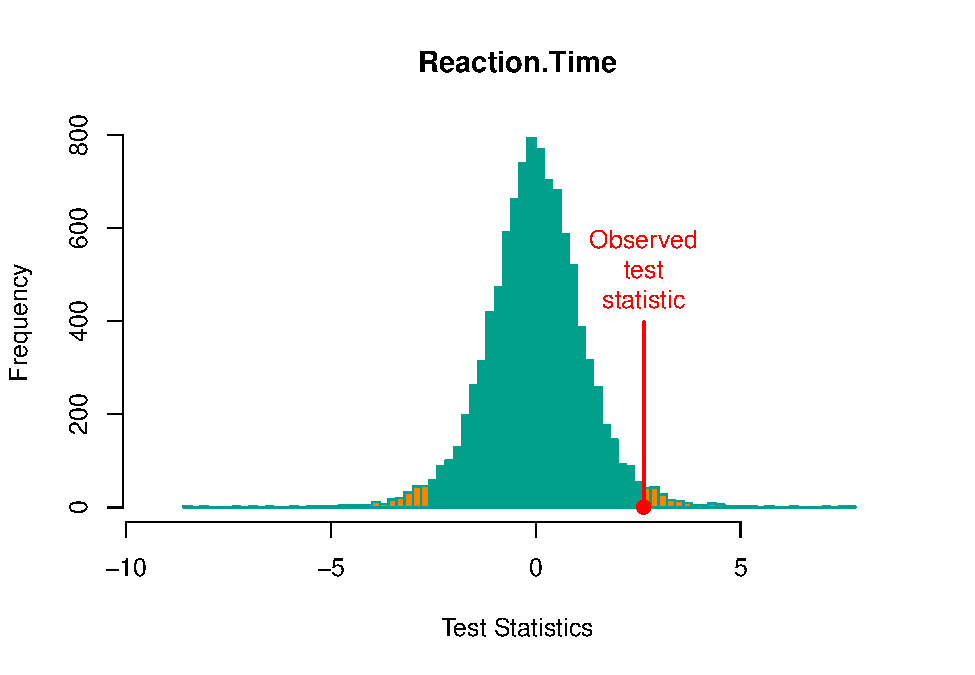
\includegraphics{perm_files/figure-latex/unnamed-chunk-17-1} \end{center}

\hypertarget{the-simple-linear-parametric-model}{%
\subsubsection{The (simple) linear parametric
model}\label{the-simple-linear-parametric-model}}

We assume that the observed values are distributed around true values
\(\beta_0 + \beta_1 X\) according to a Gaussian law:

\(Y=\textrm{linear part} + \textrm{normal error}\)

\(Y=\beta_0 + \beta_1 X + \varepsilon\)

\textbf{Assumptions of the linear model }

\begin{itemize}
\tightlist
\item
  the \(\boldsymbol{y_i=\beta_0 + \beta_1 x_i + \varepsilon_i}\) the
  relationship between X and Y is truly linear, less than the error term
  \(\varepsilon_i\)
\item
  \(\boldsymbol{\varepsilon_i \sim N (0, \sigma ^ 2), \ \forall i=1, \ldots, n}\)
  errors have normal distribution with zero mean and common variance
  (homoschedasticity: same variance).
\end{itemize}

\hypertarget{hypothesis-testing}{%
\subsubsection{Hypothesis testing}\label{hypothesis-testing}}

If these assumptions are true,

\(\hat{\beta_1} \sim N (\beta_1, \sigma ^ 2 / \sum (x_i- \bar{x}) ^ 2)\)

We calculate the test statistic:

\(t=\frac{\hat{\beta_1}}{std.dev\ \hat{\beta_1}}=\frac{\hat{\beta_1}}{\sqrt{\sum_{i=1} ^ n (y_i- \hat{y}_i) ^ 2 / \sum (x_i- \bar{x}) ^ 2 / (n-2)}}\)

If \(H_0: \beta_1=0\), \(t \sim t (n-2)\) is true

On \texttt{reaction} data and \(H_1: \beta_1 \neq 0\) (bilateral
alternative)

\begin{Shaded}
\begin{Highlighting}[]
\NormalTok{model}\OtherTok{=}\FunctionTok{lm}\NormalTok{ (Reaction.Time }\SpecialCharTok{\textasciitilde{}}\NormalTok{ Age, }\AttributeTok{data=}\NormalTok{reaction)}
\FunctionTok{summary}\NormalTok{ (model)}
\end{Highlighting}
\end{Shaded}

\begin{verbatim}
## 
## Call:
## lm(formula = Reaction.Time ~ Age, data = reaction)
## 
## Residuals:
##    Min     1Q Median     3Q    Max 
## -6.535 -3.364 -0.272  2.676  7.839 
## 
## Coefficients:
##             Estimate Std. Error t value Pr(>|t|)  
## (Intercept) 10.30135    4.04407   2.547   0.0343 *
## Age          0.20647    0.07841   2.633   0.0300 *
## ---
## Signif. codes:  0 '***' 0.001 '**' 0.01 '*' 0.05 '.' 0.1 ' ' 1
## 
## Residual standard error: 4.678 on 8 degrees of freedom
## Multiple R-squared:  0.4643, Adjusted R-squared:  0.3973 
## F-statistic: 6.934 on 1 and 8 DF,  p-value: 0.03003
\end{verbatim}

Similar result, but much more assumptions!

\hypertarget{assumptions-of-a-permutation-test}{%
\subsubsection{Assumptions of a permutation
test}\label{assumptions-of-a-permutation-test}}

What model do we assume in a permutation test?

Under the null hypo: \(H_0:\ f(y)=f(y|x) \ \forall x\)

Under the alternative hypo no assumptions. in order to have power we
hope that:

\(H_1:\ E(y|x)=\beta_0 + \beta_1x; \textrm{ with } \beta_1\neq 0 \textrm{ and for some } x\)\\
that is:\\
\(H_1: E(yx)\neq E(x)E(y)\)

No other assumptions on the distribution of \(f(y|x)\) (normality, nor
finite moments)

\hypertarget{permutationally-equivalent-tests}{%
\subsection{Permutationally equivalent
tests}\label{permutationally-equivalent-tests}}

\begin{Shaded}
\begin{Highlighting}[]
\FunctionTok{set.seed}\NormalTok{(}\DecValTok{1}\NormalTok{)}
\NormalTok{(}\AttributeTok{res\_cor=}\FunctionTok{flip}\NormalTok{(Reaction.Time}\SpecialCharTok{\textasciitilde{}}\NormalTok{Age,}\AttributeTok{data=}\NormalTok{reaction,}\AttributeTok{statTest =} \StringTok{"cor"}\NormalTok{))}
\end{Highlighting}
\end{Shaded}

\begin{verbatim}
## 
##               Test   Stat tail p-value
## Reaction.Time  cor 0.6814   ><  0.0410
\end{verbatim}

\begin{Shaded}
\begin{Highlighting}[]
\FunctionTok{set.seed}\NormalTok{(}\DecValTok{1}\NormalTok{)}
\NormalTok{(}\AttributeTok{res\_t=}\FunctionTok{flip}\NormalTok{(Reaction.Time}\SpecialCharTok{\textasciitilde{}}\NormalTok{Age,}\AttributeTok{data=}\NormalTok{reaction,}\AttributeTok{statTest =} \StringTok{"t"}\NormalTok{))}
\end{Highlighting}
\end{Shaded}

\begin{verbatim}
## 
##               Test  Stat tail p-value
## Reaction.Time    t 2.633   ><  0.0410
\end{verbatim}

\begin{Shaded}
\begin{Highlighting}[]
\FunctionTok{plot}\NormalTok{(res\_cor}\SpecialCharTok{@}\NormalTok{permT,res\_t}\SpecialCharTok{@}\NormalTok{permT,}\AttributeTok{pch=}\DecValTok{20}\NormalTok{,}\AttributeTok{col=}\DecValTok{2}\NormalTok{)}
\end{Highlighting}
\end{Shaded}

\begin{center}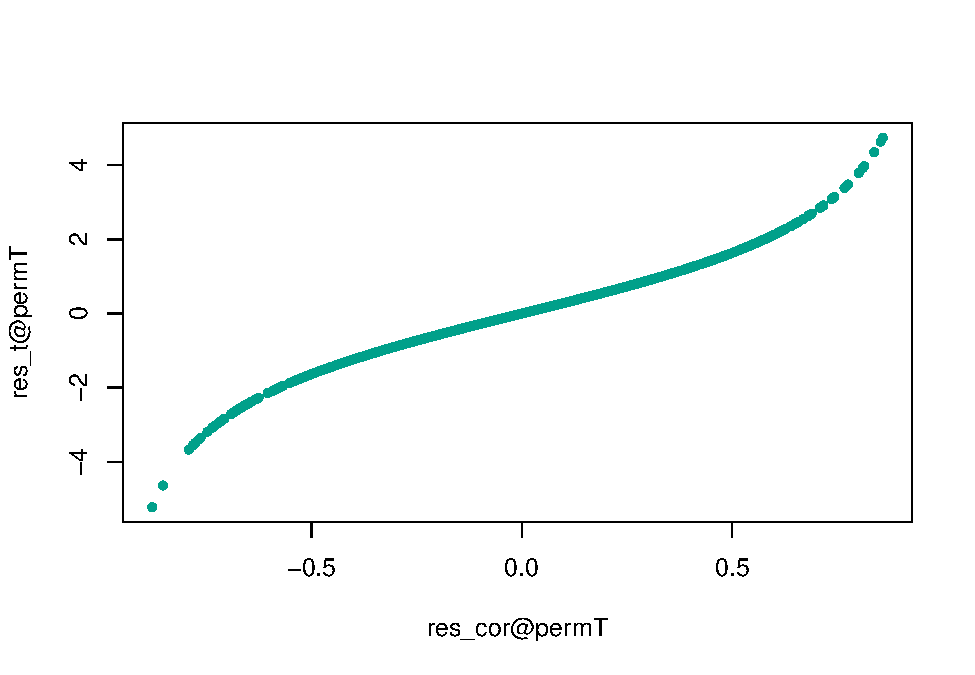
\includegraphics{perm_files/figure-latex/unnamed-chunk-19-1} \end{center}

\hypertarget{conclusion}{%
\subsubsection{Conclusion}\label{conclusion}}

\textbf{The permutation tests}:

\begin{itemize}
\tightlist
\item
  Different from bootstrap methods. The former are extractions without
  reintegration, the latter with. The former have almost optimal
  properties and have (almost always) an exact control of the first type
  errors.
\item
  They constitute a general approach and are applicable in many
  contexts. Very few assumptions.\\
\item
  some dedicated R packages:

  \begin{itemize}
  \tightlist
  \item
    \texttt{coin}
    \url{http://cran.r-project.org/web/packages/coin/index.html}
  \item
    \texttt{permuco}
    \url{https://cran.r-project.org/web/packages/permuco/index.html}
  \item
    \texttt{flip}
    \url{http://cran.r-project.org/web/packages/flip/index.html} (the
    development version is on github
    \url{https://github.com/livioivil/flip})
  \item
    \texttt{flipscores}
    \url{http://cran.r-project.org/web/packages/flipscores/index.html}
    (the development version is on github
    \url{https://github.com/livioivil/flipscores})
  \item
    \texttt{multcomp}
    \url{https://cran.r-project.org/web/packages/multcomp/index.html}
  \item
    \texttt{GFD}
    \url{https://cran.r-project.org/web/packages/GFD/index.html}
  \end{itemize}
\end{itemize}

\hypertarget{some-special-cases}{%
\section{Some special cases}\label{some-special-cases}}

\hypertarget{rank-correlation}{%
\subsection{Rank-correlation}\label{rank-correlation}}

\begin{itemize}
\tightlist
\item
  \(n\) observations from \(y\), we are interested on \(F(y|x)\)

  \begin{itemize}
  \tightlist
  \item
    we don't need \(y_1\) and \(y_2\) do be continuous, we don't even
    need to have finite moments (usual minimal assumption).
  \end{itemize}
\item
  Hypotheses

  \begin{itemize}
  \tightlist
  \item
    \(H_0: F(y|x)=F(y|x')\ \forall x,x'\)\\
  \item
    \(H_1: \exists \ x< x' : F(y|x)< F(y|x')\) or directional such as:
    \(H_1: \exists x,x' F(y_1)\neq F(y_2)\)
  \end{itemize}
\item
  Test Statistic: rank-correlation
\end{itemize}

\begin{Shaded}
\begin{Highlighting}[]
\NormalTok{(}\AttributeTok{res=}\FunctionTok{flip}\NormalTok{(Reaction.Time}\SpecialCharTok{\textasciitilde{}}\NormalTok{Age,}\AttributeTok{data=}\NormalTok{reaction,}\AttributeTok{perms =} \DecValTok{10000}\NormalTok{,}\AttributeTok{statTest  =} \StringTok{"rank"}\NormalTok{))}
\end{Highlighting}
\end{Shaded}

\begin{verbatim}
## 
##                   Test  Stat tail p-value
## Reaction.Time Wilcoxon 2.179   ><  0.0210
\end{verbatim}

\begin{Shaded}
\begin{Highlighting}[]
\CommentTok{\# to see the rank correlation use the workaround:}
\NormalTok{(}\AttributeTok{res=}\FunctionTok{flip}\NormalTok{(}\FunctionTok{rank}\NormalTok{(reaction}\SpecialCharTok{$}\NormalTok{Reaction.Time)}\SpecialCharTok{\textasciitilde{}}\FunctionTok{rank}\NormalTok{(reaction}\SpecialCharTok{$}\NormalTok{Age),}\AttributeTok{perms =} \DecValTok{10000}\NormalTok{,}\AttributeTok{statTest  =} \StringTok{"cor"}\NormalTok{))}
\end{Highlighting}
\end{Shaded}

\begin{verbatim}
## 
##                              Test   Stat tail p-value
## rank.reaction.Reaction.Time.  cor 0.7153   ><  0.0221
\end{verbatim}

\begin{Shaded}
\begin{Highlighting}[]
\NormalTok{(}\FunctionTok{cor.test}\NormalTok{(reaction}\SpecialCharTok{$}\NormalTok{Reaction.Time,reaction}\SpecialCharTok{$}\NormalTok{Age,}\AttributeTok{method=}\StringTok{"spe"}\NormalTok{))}
\end{Highlighting}
\end{Shaded}

\begin{verbatim}
## Warning in cor.test.default(reaction$Reaction.Time, reaction$Age, method =
## "spe"): Cannot compute exact p-value with ties
\end{verbatim}

\begin{verbatim}
## 
##  Spearman's rank correlation rho
## 
## data:  reaction$Reaction.Time and reaction$Age
## S = 46.983, p-value = 0.02005
## alternative hypothesis: true rho is not equal to 0
## sample estimates:
##      rho 
## 0.715256
\end{verbatim}

\begin{Shaded}
\begin{Highlighting}[]
\FunctionTok{plot}\NormalTok{(res)}
\end{Highlighting}
\end{Shaded}

\begin{center}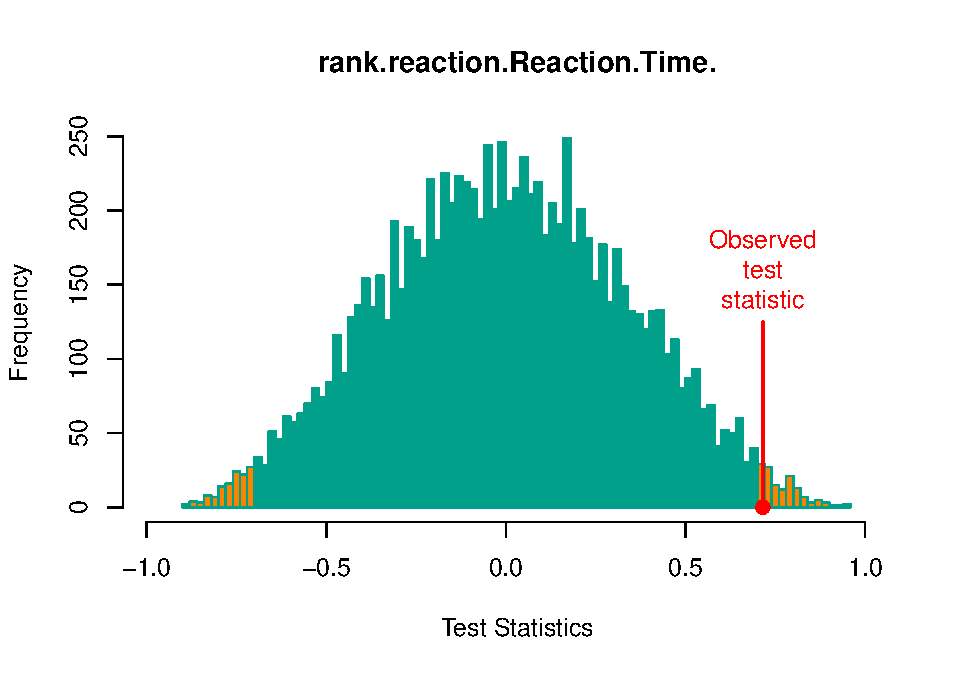
\includegraphics{perm_files/figure-latex/unnamed-chunk-21-1} \end{center}

\hypertarget{the-two-independent-sample-problem}{%
\subsection{The Two-independent-sample
problem}\label{the-two-independent-sample-problem}}

\begin{itemize}
\tightlist
\item
  Two samples:

  \begin{itemize}
  \tightlist
  \item
    \(n_1\) observations from \(y_1\)\\
  \item
    \(n_2\) observations from \(y_2\)\\
  \item
    we don't need \(y_1\) and \(y_2\) do be continuous, we don't even
    neeD to have second (nor higher order) finite moments, which is the
    usual minimal assumption.
  \end{itemize}
\item
  Hypotheses

  \begin{itemize}
  \tightlist
  \item
    \(H_0: F(y_1)=F(y_2)\)\\
  \item
    \(H_1: F(y_1)\neq F(y_2)\)\\
    (or directional such as: \(H_1: F(y_1)<F(y_2)\))
  \end{itemize}
\end{itemize}

\begin{itemize}
\tightlist
\item
  Test Statistic:

  \begin{itemize}
  \tightlist
  \item
    Standardized mean difference (t-statistic)\\
  \item
    Estimated slope coefficient (label of groups as dummy predictor)\\
  \item
    other test statistic such as the (non standardized) mean difference
    are permutationally equivalent
  \end{itemize}
\end{itemize}

\begin{Shaded}
\begin{Highlighting}[]
\FunctionTok{data}\NormalTok{(}\StringTok{"seeds"}\NormalTok{)}
\NormalTok{seeds}\OtherTok{=}\FunctionTok{na.omit}\NormalTok{(seeds)}

\NormalTok{(}\AttributeTok{res=}\FunctionTok{flip}\NormalTok{(y}\SpecialCharTok{\textasciitilde{}}\NormalTok{grp,}\AttributeTok{data=}\NormalTok{seeds,}\AttributeTok{perms =} \DecValTok{10000}\NormalTok{))}
\end{Highlighting}
\end{Shaded}

\begin{verbatim}
## 
##   Test  Stat tail p-value
## y    t 2.061   ><  0.0511
\end{verbatim}

\begin{Shaded}
\begin{Highlighting}[]
\NormalTok{(}\FunctionTok{summary}\NormalTok{(}\FunctionTok{lm}\NormalTok{(y}\SpecialCharTok{\textasciitilde{}}\NormalTok{grp,}\AttributeTok{data=}\NormalTok{seeds)))}
\end{Highlighting}
\end{Shaded}

\begin{verbatim}
## 
## Call:
## lm(formula = y ~ grp, data = seeds)
## 
## Residuals:
##    Min     1Q Median     3Q    Max 
## -7.331 -2.931 -1.651  4.663  7.863 
## 
## Coefficients:
##             Estimate Std. Error t value Pr(>|t|)    
## (Intercept)   10.147      1.242   8.168    9e-09 ***
## grp            3.345      1.623   2.061    0.049 *  
## ---
## Signif. codes:  0 '***' 0.001 '**' 0.01 '*' 0.05 '.' 0.1 ' ' 1
## 
## Residual standard error: 4.303 on 27 degrees of freedom
## Multiple R-squared:  0.136,  Adjusted R-squared:  0.104 
## F-statistic: 4.249 on 1 and 27 DF,  p-value: 0.04903
\end{verbatim}

\begin{Shaded}
\begin{Highlighting}[]
\FunctionTok{plot}\NormalTok{(res)}
\end{Highlighting}
\end{Shaded}

\begin{center}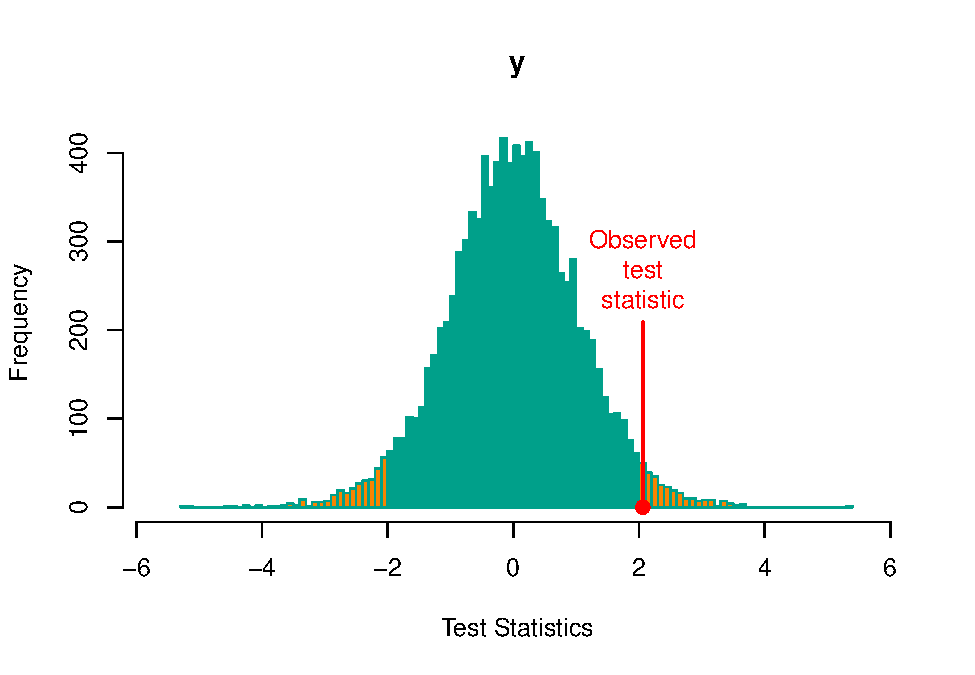
\includegraphics{perm_files/figure-latex/unnamed-chunk-23-1} \end{center}

\hypertarget{rank-test}{%
\subsubsection{Rank test}\label{rank-test}}

Can we use rank-based statistics?

Yes, equivalent to rank-tests, we just rely on exact distribution
instead of asymptotic one (and we have no limitations with ties).

\begin{Shaded}
\begin{Highlighting}[]
\NormalTok{(}\AttributeTok{res=}\FunctionTok{flip}\NormalTok{(y}\SpecialCharTok{\textasciitilde{}}\NormalTok{grp,}\AttributeTok{data=}\NormalTok{seeds,}\AttributeTok{statTest =} \StringTok{"rank"}\NormalTok{,}\AttributeTok{perms=}\DecValTok{10000}\NormalTok{))}
\end{Highlighting}
\end{Shaded}

\begin{verbatim}
## 
##       Test Stat tail p-value
## y Wilcoxon 2.13   ><  0.0317
\end{verbatim}

\begin{Shaded}
\begin{Highlighting}[]
\NormalTok{(}\FunctionTok{wilcox.test}\NormalTok{(y}\SpecialCharTok{\textasciitilde{}}\NormalTok{grp,}\AttributeTok{data=}\NormalTok{seeds))}
\end{Highlighting}
\end{Shaded}

\begin{verbatim}
## Warning in wilcox.test.default(x = c(12.54, 14.81, 16.71, 7.53, 7.02, 8.09, :
## cannot compute exact p-value with ties
\end{verbatim}

\begin{verbatim}
## 
##  Wilcoxon rank sum test with continuity correction
## 
## data:  y by grp
## W = 53.5, p-value = 0.03353
## alternative hypothesis: true location shift is not equal to 0
\end{verbatim}

\hypertarget{chi-square-and-other-cathegorical-methods}{%
\subsection{Chi square and other cathegorical
methods}\label{chi-square-and-other-cathegorical-methods}}

\begin{Shaded}
\begin{Highlighting}[]
\FunctionTok{data}\NormalTok{(}\StringTok{"seeds"}\NormalTok{)}
\NormalTok{seeds}\SpecialCharTok{$}\NormalTok{Germinated}\OtherTok{=}\SpecialCharTok{!}\FunctionTok{is.na}\NormalTok{(seeds}\SpecialCharTok{$}\NormalTok{x)}
\NormalTok{seeds}\SpecialCharTok{$}\NormalTok{Germinated}\OtherTok{=}\FunctionTok{factor}\NormalTok{(seeds}\SpecialCharTok{$}\NormalTok{Germinated)}
\NormalTok{seeds}\SpecialCharTok{$}\NormalTok{grp}\OtherTok{=}\FunctionTok{factor}\NormalTok{(seeds}\SpecialCharTok{$}\NormalTok{grp)}


\FunctionTok{table}\NormalTok{(seeds}\SpecialCharTok{$}\NormalTok{grp,seeds}\SpecialCharTok{$}\NormalTok{Germinated)}
\end{Highlighting}
\end{Shaded}

\begin{verbatim}
##    
##     FALSE TRUE
##   0     8   12
##   1     3   17
\end{verbatim}

\begin{Shaded}
\begin{Highlighting}[]
\FunctionTok{chisq.test}\NormalTok{(seeds}\SpecialCharTok{$}\NormalTok{grp,seeds}\SpecialCharTok{$}\NormalTok{Germinated)}
\end{Highlighting}
\end{Shaded}

\begin{verbatim}
## 
##  Pearson's Chi-squared test with Yates' continuity correction
## 
## data:  seeds$grp and seeds$Germinated
## X-squared = 2.0063, df = 1, p-value = 0.1567
\end{verbatim}

\begin{Shaded}
\begin{Highlighting}[]
\NormalTok{(}\AttributeTok{res=}\FunctionTok{flip}\NormalTok{(Germinated}\SpecialCharTok{\textasciitilde{}}\NormalTok{grp,}\AttributeTok{data=}\NormalTok{seeds,}\AttributeTok{statTest =} \StringTok{"Chisq"}\NormalTok{,}\AttributeTok{perms=}\DecValTok{10000}\NormalTok{))}
\end{Highlighting}
\end{Shaded}

\begin{verbatim}
## 
##                         Test  Stat tail p-value
## grp_|_Germinated Chi Squared 3.135    >  0.1557
\end{verbatim}

\begin{Shaded}
\begin{Highlighting}[]
\FunctionTok{plot}\NormalTok{(res)}
\end{Highlighting}
\end{Shaded}

\begin{center}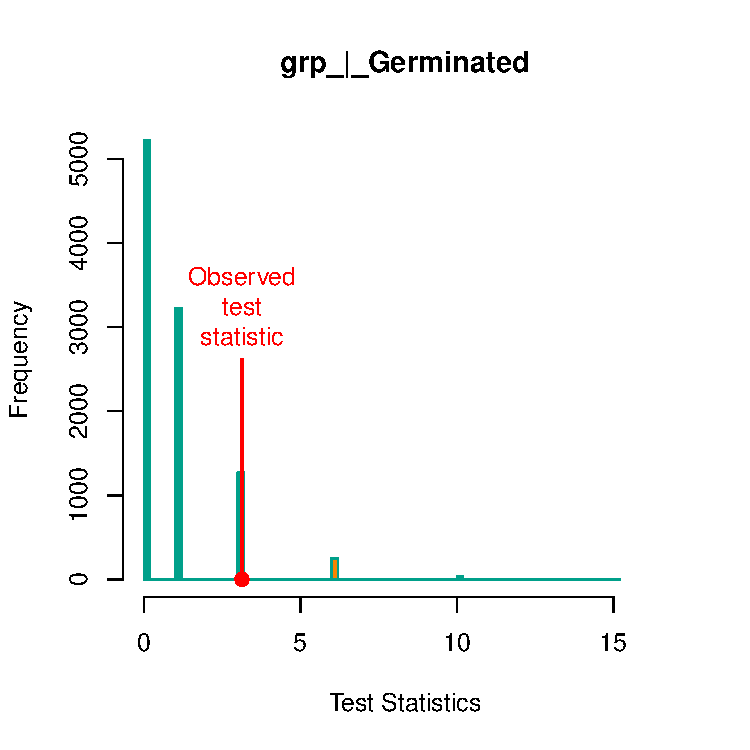
\includegraphics{perm_files/figure-latex/unnamed-chunk-27-1} \end{center}

\ldots{} and the Fisher test:

\begin{Shaded}
\begin{Highlighting}[]
\FunctionTok{fisher.test}\NormalTok{(seeds}\SpecialCharTok{$}\NormalTok{grp,seeds}\SpecialCharTok{$}\NormalTok{Germinated)}\SpecialCharTok{$}\NormalTok{p.value}
\end{Highlighting}
\end{Shaded}

\begin{verbatim}
## [1] 0.1551874
\end{verbatim}

\begin{Shaded}
\begin{Highlighting}[]
\NormalTok{(}\FunctionTok{flip}\NormalTok{(Germinated}\SpecialCharTok{\textasciitilde{}}\NormalTok{grp,}\AttributeTok{data=}\NormalTok{seeds,}\AttributeTok{perms=}\DecValTok{10000}\NormalTok{))}
\end{Highlighting}
\end{Shaded}

\begin{verbatim}
## 
##                 Test   Stat tail p-value
## GerminatedFALSE    t -1.798   ><  0.1542
## GerminatedTRUE     t  1.798   ><  0.1542
\end{verbatim}

\hypertarget{anova-c-sample}{%
\subsection{ANOVA (C-sample)}\label{anova-c-sample}}

e.g.~3 groups of \texttt{Age}: young {[}18-35), middle age {[}35-60),
old {[}60-100)

\begin{itemize}
\tightlist
\item
  C samples:

  \begin{itemize}
  \tightlist
  \item
    \(n_i\) observations from \(y_i\) (\(i=1,\ldots,C\))
  \item
    we don't need \(y_i\) do be continuous, we don't even need to have
    finite moments (usual minimal assumption)
  \end{itemize}
\item
  Hypotheses

  \begin{itemize}
  \tightlist
  \item
    \(H_0: F(y_i)=F(y_j)\ \forall (i,j)\)\\
  \item
    \(H_1: \exists (i,j): \ F(y_i)\neq F(y_j)\)
  \end{itemize}
\end{itemize}

\begin{itemize}
\tightlist
\item
  Test Statistic:

  \begin{itemize}
  \tightlist
  \item
    F-statistic\\
  \item
    \(R^2\)\\
  \item
    other test statistic such as the (non standardized) mean difference
    are permutationally equivalent
  \item
    Rank-based is also possible
  \end{itemize}
\end{itemize}

\begin{Shaded}
\begin{Highlighting}[]
\NormalTok{reaction}\SpecialCharTok{$}\NormalTok{AgeCateg}\OtherTok{=}\FunctionTok{cut}\NormalTok{(reaction}\SpecialCharTok{$}\NormalTok{Age,}\FunctionTok{c}\NormalTok{(}\DecValTok{18}\NormalTok{,}\DecValTok{35}\NormalTok{,}\DecValTok{65}\NormalTok{,}\DecValTok{100}\NormalTok{),}\AttributeTok{right =} \ConstantTok{FALSE}\NormalTok{)}
  
\NormalTok{(}\AttributeTok{res=}\FunctionTok{flip}\NormalTok{(Reaction.Time}\SpecialCharTok{\textasciitilde{}}\NormalTok{AgeCateg,}\AttributeTok{data=}\NormalTok{reaction,}\AttributeTok{perms =} \DecValTok{10000}\NormalTok{,}\AttributeTok{statTest  =} \StringTok{"ANOVA"}\NormalTok{))}
\end{Highlighting}
\end{Shaded}

\begin{verbatim}
## 
##               Test Stat tail p-value
## Reaction.Time    F 4.02    >  0.0838
\end{verbatim}

\begin{Shaded}
\begin{Highlighting}[]
\FunctionTok{summary}\NormalTok{(}\FunctionTok{lm}\NormalTok{(Reaction.Time}\SpecialCharTok{\textasciitilde{}}\NormalTok{AgeCateg,}\AttributeTok{data=}\NormalTok{reaction))}
\end{Highlighting}
\end{Shaded}

\begin{verbatim}
## 
## Call:
## lm(formula = Reaction.Time ~ AgeCateg, data = reaction)
## 
## Residuals:
##    Min     1Q Median     3Q    Max 
## -6.495 -3.279  0.465  2.246  6.112 
## 
## Coefficients:
##                  Estimate Std. Error t value Pr(>|t|)    
## (Intercept)        16.157      2.331   6.932 0.000225 ***
## AgeCateg[35,65)     4.428      3.296   1.343 0.221144    
## AgeCateg[65,100)   11.418      4.037   2.828 0.025478 *  
## ---
## Signif. codes:  0 '***' 0.001 '**' 0.01 '*' 0.05 '.' 0.1 ' ' 1
## 
## Residual standard error: 4.662 on 7 degrees of freedom
## Multiple R-squared:  0.5346, Adjusted R-squared:  0.4016 
## F-statistic:  4.02 on 2 and 7 DF,  p-value: 0.06878
\end{verbatim}

\hypertarget{stochastic-ordering}{%
\subsubsection{Stochastic Ordering}\label{stochastic-ordering}}

\begin{itemize}
\tightlist
\item
  Same assumptions of ANOVA\\
\item
  Hypotheses

  \begin{itemize}
  \tightlist
  \item
    same null hypo \(H_0: F(y_i)=F(y_j)\ \forall (i,j)\)\\
  \item
    BUT \(H_1: \exists (i,j): \ F(y_i)< F(y_j)\) (or \(>\))
  \end{itemize}
\end{itemize}

(more details on NPC later)

\begin{Shaded}
\begin{Highlighting}[]
\NormalTok{(}\AttributeTok{res=}\FunctionTok{flip}\NormalTok{(Reaction.Time}\SpecialCharTok{\textasciitilde{}}\NormalTok{AgeCateg,}\AttributeTok{data=}\NormalTok{reaction,}\AttributeTok{perms =} \DecValTok{10000}\NormalTok{,}\AttributeTok{tail=}\DecValTok{1}\NormalTok{))}
\end{Highlighting}
\end{Shaded}

\begin{verbatim}
## 
##                                    Test   Stat tail p-value
## Reaction.Time_|_AgeCateg.[35,65).     t 0.1423    >  0.4322
## Reaction.Time_|_AgeCateg.[65,100).    t 2.2444    >  0.0259
\end{verbatim}

\begin{Shaded}
\begin{Highlighting}[]
\FunctionTok{npc}\NormalTok{(res)}
\end{Highlighting}
\end{Shaded}

\begin{verbatim}
## 
##    comb.funct nVar  Stat p-value
## V1     Fisher    2 4.492  0.0210
\end{verbatim}

\hypertarget{stratified-permutations-discrete-nuisances}{%
\subsection{Stratified permutations (discrete
nuisances)}\label{stratified-permutations-discrete-nuisances}}

What if we want to test \(x=\) \texttt{Age} also using \(z=\)
\texttt{Gender} as nuisance in the \texttt{reaction} data set?

Under the null hypothesis:
\(f(y|x,z)=f(y|x',z)=f(y|z) \ \forall (x,x')\)

Therefore, even under the \(H_0\), it holds \(f(y_i)=f(y_j)\) ONLY IF
\(z_i=z_j\) (obs \(i\) and \(j\) have the same gender).

Can e permute same as in the previous cases? NO. We permute the
observations only within the strata defined by \(z\).

\textbf{Remark}:\\
- we don't assume linear effect of the nuisance,\\
- we also allow heteroscedastic errors among strata.

(Test statistic remains the same)

\begin{Shaded}
\begin{Highlighting}[]
\NormalTok{(}\AttributeTok{res=}\FunctionTok{flip}\NormalTok{(Reaction.Time}\SpecialCharTok{\textasciitilde{}}\NormalTok{Age,}\AttributeTok{Strata=}\SpecialCharTok{\textasciitilde{}}\NormalTok{Gender,}\AttributeTok{data=}\NormalTok{reaction,}\AttributeTok{perms=}\DecValTok{10000}\NormalTok{))}
\end{Highlighting}
\end{Shaded}

\begin{verbatim}
## 
##               Test  Stat tail p-value
## Reaction.Time    t 2.633   ><  0.0684
\end{verbatim}

Alternative model (more about NPC later):

\begin{Shaded}
\begin{Highlighting}[]
\NormalTok{(}\AttributeTok{res=}\FunctionTok{flip}\NormalTok{(Reaction.Time}\SpecialCharTok{\textasciitilde{}}\NormalTok{Age}\SpecialCharTok{*}\NormalTok{Gender,}\AttributeTok{Strata=}\SpecialCharTok{\textasciitilde{}}\NormalTok{Gender,}\AttributeTok{data=}\NormalTok{reaction,}\AttributeTok{perms=}\DecValTok{10000}\NormalTok{))}
\end{Highlighting}
\end{Shaded}

\begin{verbatim}
## 
##                               Test    Stat tail p-value
## Reaction.Time_|_Age              t  2.4826   ><  0.0725
## Reaction.Time_|_Age:Gender.M.    t -0.6518   ><  0.3402
\end{verbatim}

\begin{Shaded}
\begin{Highlighting}[]
\FunctionTok{npc}\NormalTok{(res)}
\end{Highlighting}
\end{Shaded}

\begin{verbatim}
## 
##    comb.funct nVar  Stat p-value
## V1     Fisher    2 3.702  0.1371
\end{verbatim}

\hypertarget{multivariate-testing}{%
\section{Multivariate Testing}\label{multivariate-testing}}

\hypertarget{seeds-data}{%
\subsection{Seeds data}\label{seeds-data}}

\begin{Shaded}
\begin{Highlighting}[]
\CommentTok{\# install.packages("flip")}
\FunctionTok{library}\NormalTok{(flip)}
\end{Highlighting}
\end{Shaded}

omit the \texttt{NA}s:

\begin{Shaded}
\begin{Highlighting}[]
\FunctionTok{data}\NormalTok{(seeds,}\AttributeTok{package =} \StringTok{"flip"}\NormalTok{)}
\NormalTok{seeds}\OtherTok{=}\FunctionTok{na.omit}\NormalTok{(seeds)}
\NormalTok{seeds}
\end{Highlighting}
\end{Shaded}

\begin{verbatim}
##    grp    x     y
## 9    0 6.03 12.54
## 10   0 4.20 14.81
## 11   0 4.49 16.71
## 12   0 2.00  7.53
## 13   0 2.84  7.02
## 14   0 3.88  8.09
## 15   0 2.04  5.76
## 16   0 5.48 18.01
## 17   0 2.31  8.81
## 18   0 1.90  8.17
## 19   0 1.75  6.62
## 20   0 3.02  7.69
## 24   1 3.31 18.49
## 25   1 6.56 19.20
## 26   1 3.16  9.85
## 27   1 4.07 15.83
## 28   1 2.09  6.16
## 29   1 6.72 17.58
## 30   1 3.93 19.29
## 31   1 2.56 10.77
## 32   1 8.30 18.31
## 33   1 4.21 10.56
## 34   1 1.86  9.48
## 35   1 3.09 12.54
## 36   1 5.09 18.35
## 37   1 4.08 11.84
## 38   1 3.63 11.44
## 39   1 2.61  7.66
## 40   1 5.21 12.00
\end{verbatim}

Use a permutation methods to test if there is any difference between the
two groups in \texttt{grp} on the two variables \texttt{x} and
\texttt{y}:

\begin{itemize}
\tightlist
\item
  perform the two tests for the two variables
\item
  Combine the two p-values using the Fisher Combining Function to test
  the global hypothesis
\item
  Use a closed testing procedure to adjust the 2 p-values.
\end{itemize}

\hypertarget{joint-distribution}{%
\subsection{Joint distribution}\label{joint-distribution}}

\begin{Shaded}
\begin{Highlighting}[]
\FunctionTok{library}\NormalTok{(flip)}
\NormalTok{res}\OtherTok{=}\FunctionTok{flip}\NormalTok{(.}\SpecialCharTok{\textasciitilde{}}\NormalTok{grp,}\AttributeTok{data=}\NormalTok{seeds)}
\FunctionTok{hist}\NormalTok{(res)}
\end{Highlighting}
\end{Shaded}

\begin{center}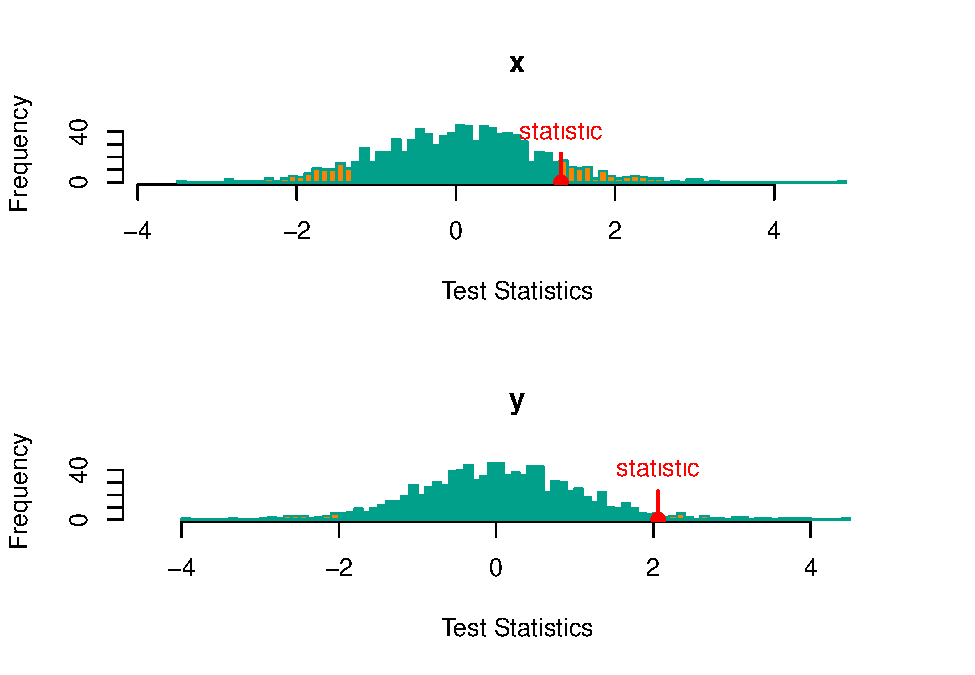
\includegraphics{perm_files/figure-latex/unnamed-chunk-35-1} \end{center}

\begin{Shaded}
\begin{Highlighting}[]
\FunctionTok{plot}\NormalTok{(res)}
\end{Highlighting}
\end{Shaded}

\begin{center}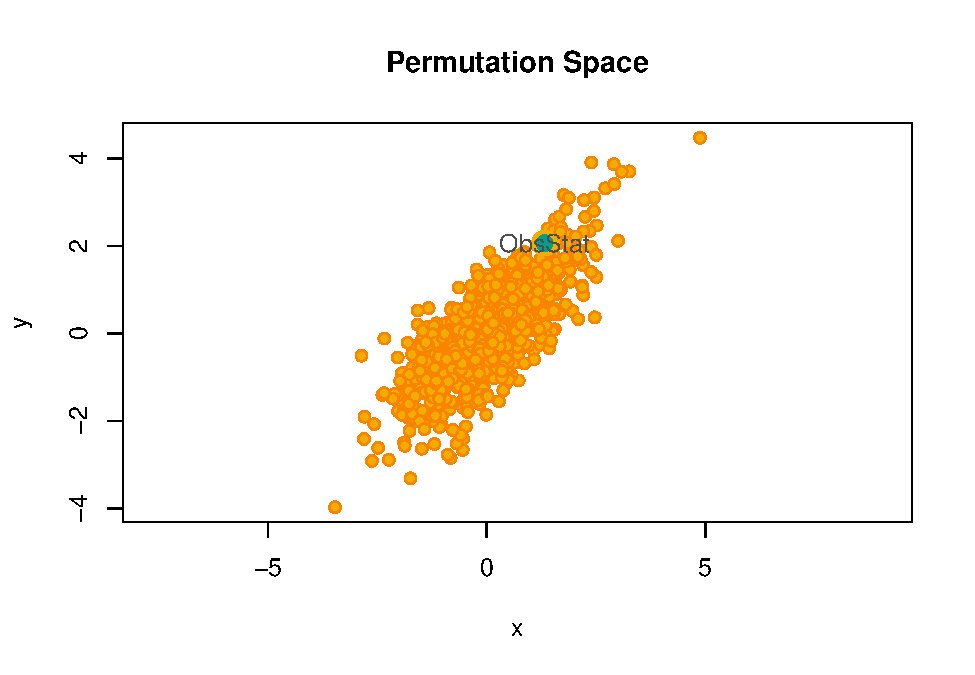
\includegraphics{perm_files/figure-latex/unnamed-chunk-35-2} \end{center}

\begin{Shaded}
\begin{Highlighting}[]
\CommentTok{\# Global p{-}value}
\FunctionTok{npc}\NormalTok{(res,}\StringTok{"Fisher"}\NormalTok{)}
\end{Highlighting}
\end{Shaded}

\begin{verbatim}
## 
##    comb.funct nVar  Stat p-value
## V1     Fisher    2 4.628  0.0880
\end{verbatim}

\begin{Shaded}
\begin{Highlighting}[]
\CommentTok{\# adjusted p: Closed testing with Fisher combination}
\FunctionTok{flip.adjust}\NormalTok{(res,}\StringTok{"Fisher"}\NormalTok{)}
\end{Highlighting}
\end{Shaded}

\begin{verbatim}
## 
##   Test  Stat tail p-value Adjust:Fisher
## x    t 1.320   ><  0.1810        0.1810
## y    t 2.061   ><  0.0540        0.0880
\end{verbatim}

\hypertarget{rejection-regions}{%
\subsection{Rejection regions}\label{rejection-regions}}

Ask for the multivariate distribution of the p-values:

\begin{Shaded}
\begin{Highlighting}[]
\NormalTok{res}\OtherTok{=}\FunctionTok{flip}\NormalTok{(.}\SpecialCharTok{\textasciitilde{}}\NormalTok{grp,}\AttributeTok{data=}\NormalTok{seeds,}\AttributeTok{flipReturn =}\FunctionTok{list}\NormalTok{(}\AttributeTok{permP=}\ConstantTok{TRUE}\NormalTok{,}\AttributeTok{permT=}\ConstantTok{TRUE}\NormalTok{))}
\NormalTok{res.fisher}\OtherTok{=}\FunctionTok{npc}\NormalTok{(res,}\StringTok{"Fisher"}\NormalTok{,}\AttributeTok{flipReturn =}\FunctionTok{list}\NormalTok{(}\AttributeTok{permP=}\ConstantTok{TRUE}\NormalTok{,}\AttributeTok{permT=}\ConstantTok{TRUE}\NormalTok{))}
\NormalTok{res.tippett}\OtherTok{=}\FunctionTok{npc}\NormalTok{(res,}\StringTok{"minP"}\NormalTok{,}\AttributeTok{flipReturn =}\FunctionTok{list}\NormalTok{(}\AttributeTok{permP=}\ConstantTok{TRUE}\NormalTok{,}\AttributeTok{permT=}\ConstantTok{TRUE}\NormalTok{))}
\end{Highlighting}
\end{Shaded}

\hypertarget{fisher-combining-function}{%
\subsubsection{Fisher Combining
Function}\label{fisher-combining-function}}

We inspect the rejection regions of the two univariate tests and the one
of Fisher combination.\\
The intersection of each univariate test with the Fisher region defines
the rejection region of a closed testing - i.e.~adjusted for multiple
testing.

\begin{center}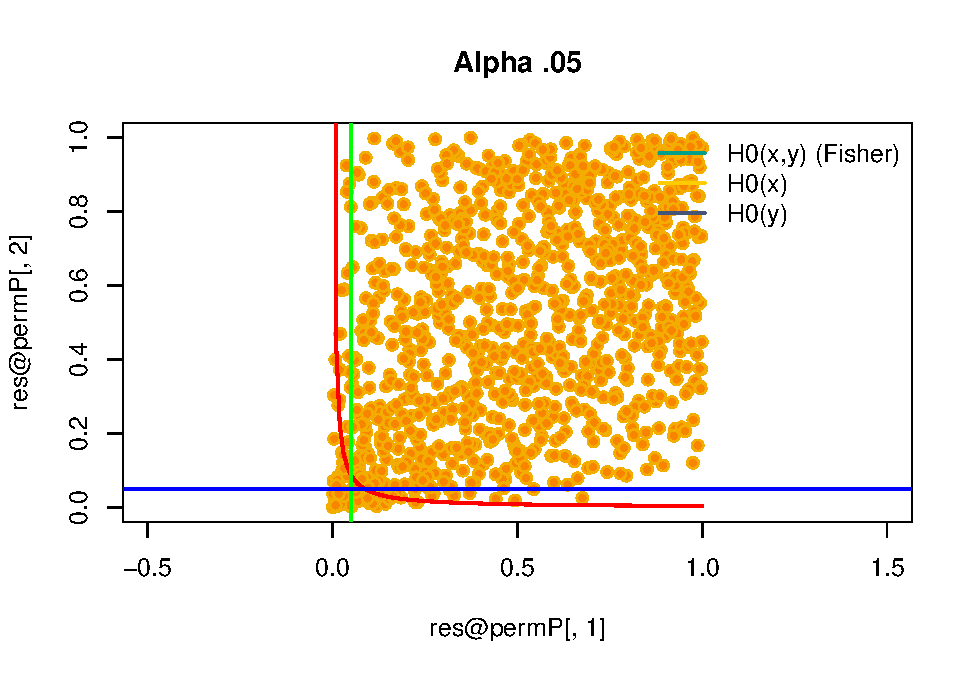
\includegraphics{perm_files/figure-latex/unnamed-chunk-37-1} \end{center}

\hypertarget{tippett-min-p-combining-function}{%
\subsubsection{Tippett (min-p) Combining
Function}\label{tippett-min-p-combining-function}}

We inspect the rejection regions of the two univariate tests and the one
of Fisher combination.\\
The intersection of each univariate test with the Fisher region defines
the rejection region of a closed testing - i.e.~adjusted for multiple
testing. This fall to be the same rejection region given by Wesfall \&
Young. Indeed, it is a closed testing with shortcut.

\begin{center}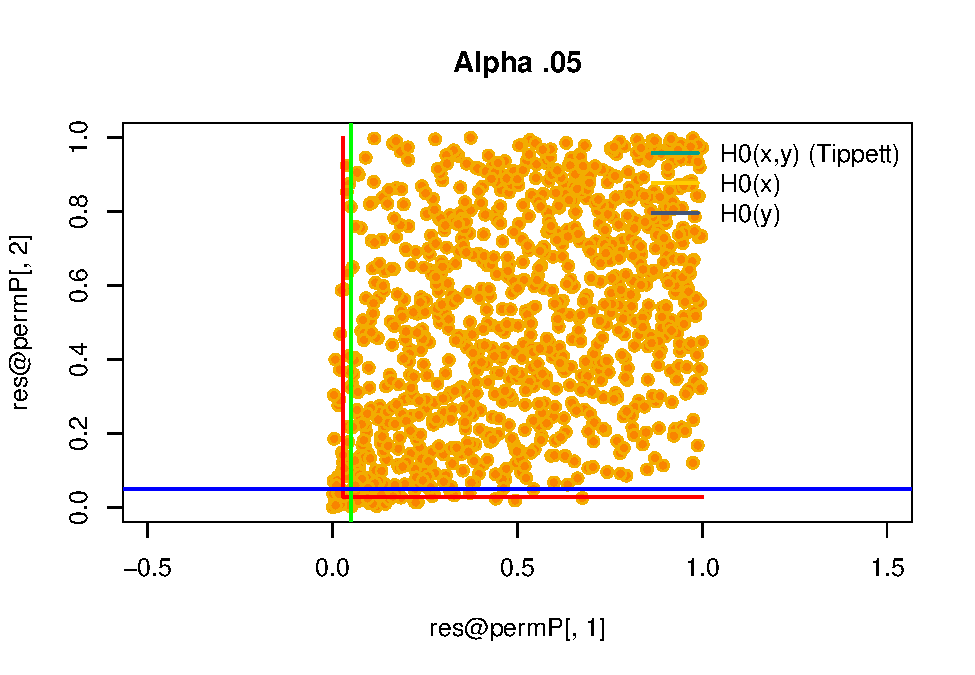
\includegraphics{perm_files/figure-latex/unnamed-chunk-38-1} \end{center}

\hypertarget{fwer-control-via-permutations-tests}{%
\section{FWER control via Permutations
tests}\label{fwer-control-via-permutations-tests}}

\hypertarget{permutation-bonferroni}{%
\subsection{Permutation Bonferroni}\label{permutation-bonferroni}}

Bonferroni is conservative

\begin{itemize}
\tightlist
\item
  \textbf{Bonferroni bound}\\
  Reject for p-values at most \(\alpha/m\)\\
\item
  \textbf{By Boole's inequality}\\
  Guaranteed: FWER \(\leq \alpha\), but often FWER \(<\alpha\)\\
\item
  \textbf{Can we improve?}\\
  Reject for p-values at most \(\tilde\alpha > \alpha/m\), while keeping
  FWER control\\
\item
  \textbf{Yes we can}\\
  By permutations
\end{itemize}

\hypertarget{improved-bonferroni}{%
\subsection{Improved Bonferroni}\label{improved-bonferroni}}

\begin{itemize}
\tightlist
\item
  \textbf{Reduced \(\alpha\)}\\
  Reject \(H_i\) if \(p_i \leq \tilde\alpha\)
\item
  \textbf{Control of FWER?}
\end{itemize}

\[
\begin{aligned}
\mathrm{FWER} &= \mathrm{P} \big(\textrm{$p_i \leq \tilde\alpha$ for at least one $i$ with $H_i$ true} \big) \\
    &= \mathrm{P} \Big( \bigcup_{i\in T} \{p_i \leq \tilde\alpha\} \Big) \\
    &= \mathrm{P} \Big( \min_{i \in T} p_i \leq \tilde\alpha \Big) \leq \alpha
\end{aligned}
\]

\begin{itemize}
\tightlist
\item
  \textbf{How can we determine the value of \(\tilde \alpha\)?}\\
  Using permutations to find the distribution of the minimum p-value
\end{itemize}

\hypertarget{multiple-testing-using-permutations}{%
\subsection{Multiple testing using
permutations}\label{multiple-testing-using-permutations}}

\textbf{The single step min-P method}

\begin{itemize}
\tightlist
\item
  Calculate the smallest p-value \(m\) for the real data\\
\item
  Randomly permute the data\\
\item
  Calculate new p-values for all tests based on permuted data\\
\item
  Calculate the smallest p-value \(m^\pi\) for permuted data\\
\item
  Repeat permutation many (say k=1000) times:
  \(m^\pi_1, \ldots, m^\pi_k\)\\
\item
  Calculate \(\tilde\alpha\) as the \(\alpha\)-quantile of
  \(m^\pi_1, \ldots, m^\pi_k\)
\end{itemize}

\textbf{Multiple testing result}\\
Reject all hypotheses with (non-permuted) p-values at most
\(\tilde\alpha\)

\hypertarget{correlation-structure-of-p-values}{%
\subsection{Correlation structure of
p-values}\label{correlation-structure-of-p-values}}

\textbf{Permutation}\\
- Destroys correlation between covariates and response\\
- Retains correlation among covariates

\textbf{Consequence}\\
- P-values of correlated tests (i.e.~data) remain correlated in
permutations\\
- Distribution of minimum p-value correctly takes correlations into
account

\textbf{When the gain relative to Bonferroni is the gain large?}\\
- Negatively correlated p-values: typically no gain\\
- Independent p-values: minimal gain\\
- Positively correlated p-values: gain can be large

\hypertarget{westfall-young-permutation-holm}{%
\subsection{Westfall \&~Young: permutation
Holm}\label{westfall-young-permutation-holm}}

\emph{Westfall PH, Young SS (1993) Resampling-Based Multiple Testing:
Examples and Methods for p-Value Adjustment. Wiley}

\textbf{Sequential permutation multiple testing}

\begin{itemize}
\tightlist
\item
  \textbf{Single step}\\
  Single step min-P is permutation equivalent of Bonferroni\\
\item
  \textbf{What about Holm?}\\
  Permutation equivalent of Holm's method: Westfall \&~Young
\end{itemize}

\textbf{The min-P algorithm}

\begin{itemize}
\tightlist
\item
  Start with all hypotheses
\item
  Repeat

  \begin{itemize}
  \tightlist
  \item
    Do single step min-P to calculate \(\tilde\alpha\)\\
  \item
    Reject hypotheses with p-value \(\leq \tilde\alpha\)\\
  \item
    Remove rejected hypotheses\\
  \end{itemize}
\item
  Until no new rejections occur
\end{itemize}

\hypertarget{closed-testing}{%
\subsection{Closed Testing}\label{closed-testing}}

\emph{R Marcus, E Peritz, KR Gabriel (1976). On closed testing
procedures with special reference to ordered analysis of variance.
Biometrika 63: 655-660.}

Test in each node: any multivariate permutation test

\hypertarget{closure-set}{%
\subsubsection{Closure Set}\label{closure-set}}

\begin{center}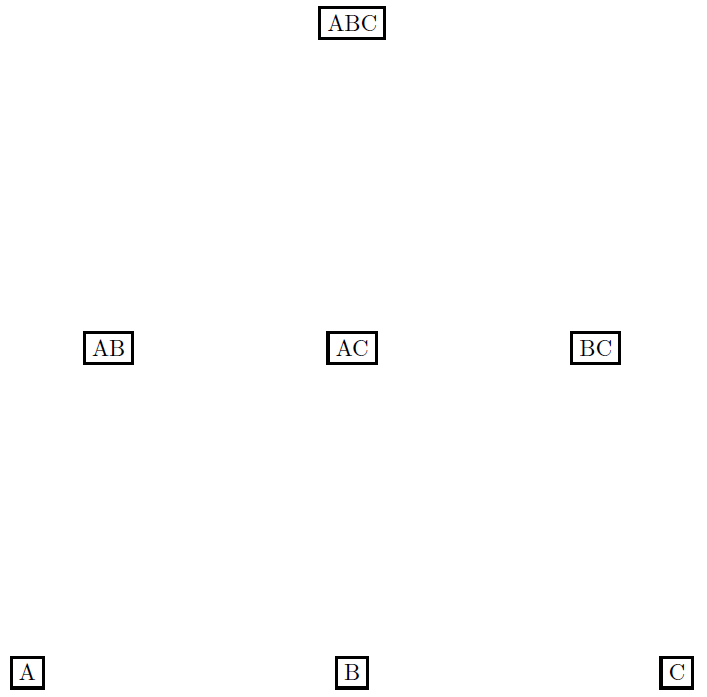
\includegraphics[width=9.82in]{./figs/closed_set} \end{center}

Adjusted \(\tilde p_A=\max(p_A,p_{AB},p_{AC},p_{ABC})\)

\hypertarget{conclusion-1}{%
\subsection{Conclusion}\label{conclusion-1}}

\textbf{Accounting for dependencies}

Adjusted p-value become lower (i.e.~more rejections)

\textbf{When?}\\
- Negative correlation: generally no gain\\
p-value Independents: little or no gain\\
- Positive correlation: big gain, usually\\
(NB: a test with bi-directional alternative and with negative
correlation produce p-value positively correlated)

\textbf{Real data}\\
The variables of real data sets are often correlated\\
then permutations are (often) convenient

\textbf{How?} \texttt{R:\ library(flip);\ flip();\ flip.adjust()}

\hypertarget{a-case-study-pharmacokinetic-study-of-carbidopa}{%
\section{A case study: Pharmacokinetic Study of
Carbidopa}\label{a-case-study-pharmacokinetic-study-of-carbidopa}}

Description:\\
\url{http://webserv.jcu.edu/math//faculty/TShort/Bradstreet/part2/part2-table6.html}

As part of a pharmacokinetic study, 12 healthy male subjects were
allocated randomly to a three period crossover design receiving one of
three graded doses (25, 50, 100 mg) of Carbidopa q8h in each treatment
period. A seven day washout period separated the treatment periods. The
pharmacokinetic variables AUC, Cmax, and Tmax were calculated for each
subject from plasma concentrations assayed from blood samples taken at
0, 0.5, 1, 1.5, 2, 3, 4, 5, 6, 7, and 8 hours postdosing following the
second dose of carbidopa on the sixth day of each treatment period.

dataset:\\
\url{http://webserv.jcu.edu/math//faculty/TShort/Bradstreet/part2/Bradp2t6.txt}

Analyze the dataset without taking in account the Study Periods (which
have been randomized in each subject, hence we can avoid to account for
it in the analysis).

Research questions:

\begin{itemize}
\tightlist
\item
  Is there a dose response for AUC, Cmax, or Tmax? Overall?
\item
  Can dose proportionality be established? (try to fit a linear model
  for each endpoint, then discuss the results)
\end{itemize}

\hypertarget{a-solution}{%
\subsection{A solution}\label{a-solution}}

We answer to both first and second question with a single analysis: we
perform a linear model (accounting for individual variability) on log
transformed end-points.

\begin{Shaded}
\begin{Highlighting}[]
\CommentTok{\#Reading and make{-}up of the data}

\NormalTok{dati}\OtherTok{=}\FunctionTok{read.table}\NormalTok{(}\StringTok{"http://webserv.jcu.edu/math//faculty/TShort/Bradstreet/part2/Bradp2t6.txt"}\NormalTok{,}\AttributeTok{skip =} \DecValTok{1}\NormalTok{,}\AttributeTok{header =} \ConstantTok{TRUE}\NormalTok{)}

\NormalTok{dati}\OtherTok{=}\FunctionTok{cbind}\NormalTok{(dati[,}\DecValTok{1}\NormalTok{],}\FunctionTok{matrix}\NormalTok{(}\FunctionTok{as.matrix}\NormalTok{(dati[,}\SpecialCharTok{{-}}\DecValTok{1}\NormalTok{]),}\FunctionTok{nrow}\NormalTok{(dati)}\SpecialCharTok{*}\DecValTok{3}\NormalTok{,}\DecValTok{4}\NormalTok{))}
\FunctionTok{colnames}\NormalTok{(dati)}\OtherTok{=}\FunctionTok{c}\NormalTok{(}\StringTok{"Sub"}\NormalTok{,}\StringTok{"Dose"}\NormalTok{,}\StringTok{"AUC"}\NormalTok{,}\StringTok{"Cmax"}\NormalTok{,}\StringTok{"Tmax"}\NormalTok{)}

\NormalTok{dati}\OtherTok{=}\FunctionTok{as.data.frame}\NormalTok{(dati)}
\FunctionTok{str}\NormalTok{(dati)}
\end{Highlighting}
\end{Shaded}

\begin{verbatim}
## 'data.frame':    36 obs. of  5 variables:
##  $ Sub : num  1 2 3 4 5 6 7 8 9 10 ...
##  $ Dose: num  100 25 50 50 50 25 100 25 50 25 ...
##  $ AUC : num  604 140 386 175 605 ...
##  $ Cmax: num  137 44.4 86.6 46.4 194 44.9 318 29 119 58.4 ...
##  $ Tmax: num  1.5 1 1.5 1.5 0.5 1 1 1 2 2 ...
\end{verbatim}

\begin{Shaded}
\begin{Highlighting}[]
\CommentTok{\# transform all responses with log{-}transformed, }
\CommentTok{\# so that a linear relationship between time and end{-}point indicates proportionality }
\NormalTok{dati[,}\DecValTok{3}\SpecialCharTok{:}\DecValTok{5}\NormalTok{]}\OtherTok{=}\FunctionTok{log}\NormalTok{(dati[,}\DecValTok{3}\SpecialCharTok{:}\DecValTok{5}\NormalTok{])}
\end{Highlighting}
\end{Shaded}

\begin{Shaded}
\begin{Highlighting}[]
\CommentTok{\#Descriptives and plots:}
\FunctionTok{summary}\NormalTok{(dati[,}\SpecialCharTok{{-}}\DecValTok{1}\NormalTok{])}
\end{Highlighting}
\end{Shaded}

\begin{verbatim}
##       Dose             AUC             Cmax            Tmax        
##  Min.   : 25.00   Min.   :4.337   Min.   :3.219   Min.   :-0.6931  
##  1st Qu.: 25.00   1st Qu.:5.156   1st Qu.:3.966   1st Qu.: 0.0000  
##  Median : 50.00   Median :5.886   Median :4.485   Median : 0.2027  
##  Mean   : 58.33   Mean   :5.873   Mean   :4.547   Mean   : 0.2474  
##  3rd Qu.:100.00   3rd Qu.:6.539   3rd Qu.:5.280   3rd Qu.: 0.6931  
##  Max.   :100.00   Max.   :7.335   Max.   :5.989   Max.   : 1.0986
\end{verbatim}

\begin{Shaded}
\begin{Highlighting}[]
\FunctionTok{by}\NormalTok{(dati[,}\DecValTok{3}\SpecialCharTok{:}\DecValTok{5}\NormalTok{],dati}\SpecialCharTok{$}\NormalTok{Dose,summary)}
\end{Highlighting}
\end{Shaded}

\begin{verbatim}
## dati$Dose: 25
##       AUC             Cmax            Tmax        
##  Min.   :4.337   Min.   :3.219   Min.   :-0.6931  
##  1st Qu.:4.803   1st Qu.:3.390   1st Qu.: 0.0000  
##  Median :4.972   Median :3.801   Median : 0.0000  
##  Mean   :5.051   Mean   :3.783   Mean   : 0.2071  
##  3rd Qu.:5.289   3rd Qu.:4.022   3rd Qu.: 0.6931  
##  Max.   :5.818   Max.   :4.464   Max.   : 0.6931  
## ------------------------------------------------------------ 
## dati$Dose: 50
##       AUC             Cmax            Tmax        
##  Min.   :5.133   Min.   :3.837   Min.   :-0.6931  
##  1st Qu.:5.670   1st Qu.:4.374   1st Qu.: 0.0000  
##  Median :5.886   Median :4.484   Median : 0.2027  
##  Mean   :5.815   Mean   :4.479   Mean   : 0.1689  
##  3rd Qu.:5.967   3rd Qu.:4.625   3rd Qu.: 0.4055  
##  Max.   :6.405   Max.   :5.268   Max.   : 1.0986  
## ------------------------------------------------------------ 
## dati$Dose: 100
##       AUC             Cmax            Tmax       
##  Min.   :6.164   Min.   :4.920   Min.   :0.0000  
##  1st Qu.:6.607   1st Qu.:5.229   1st Qu.:0.0000  
##  Median :6.782   Median :5.412   Median :0.4055  
##  Mean   :6.751   Mean   :5.378   Mean   :0.3662  
##  3rd Qu.:6.922   3rd Qu.:5.515   3rd Qu.:0.6931  
##  Max.   :7.335   Max.   :5.989   Max.   :1.0986
\end{verbatim}

\begin{Shaded}
\begin{Highlighting}[]
\FunctionTok{par}\NormalTok{(}\AttributeTok{mfrow=}\FunctionTok{c}\NormalTok{(}\DecValTok{2}\NormalTok{,}\DecValTok{2}\NormalTok{))}
\FunctionTok{plot}\NormalTok{(dati}\SpecialCharTok{$}\NormalTok{Dose,dati}\SpecialCharTok{$}\NormalTok{AUC,}\AttributeTok{ylab=}\StringTok{"log(AUC)"}\NormalTok{,}\AttributeTok{xlab=}\StringTok{"Dose"}\NormalTok{,}\AttributeTok{main=}\StringTok{"Dose vs log(AUC)"}\NormalTok{)}

\NormalTok{r}\OtherTok{=}\FunctionTok{sapply}\NormalTok{(}\FunctionTok{unique}\NormalTok{(dati}\SpecialCharTok{$}\NormalTok{Sub),}\ControlFlowTok{function}\NormalTok{(s)\{}
\NormalTok{  d}\OtherTok{=}\FunctionTok{subset}\NormalTok{(dati,Sub}\SpecialCharTok{==}\NormalTok{s)}
\NormalTok{  d}\OtherTok{=}\NormalTok{d[}\FunctionTok{order}\NormalTok{(d}\SpecialCharTok{$}\NormalTok{Dose),]}
  \FunctionTok{lines}\NormalTok{(d}\SpecialCharTok{$}\NormalTok{Dose,(d}\SpecialCharTok{$}\NormalTok{AUC),}\AttributeTok{col=}\NormalTok{s,}\AttributeTok{lwd=}\DecValTok{2}\NormalTok{)\})}


\FunctionTok{plot}\NormalTok{(dati}\SpecialCharTok{$}\NormalTok{Dose,dati}\SpecialCharTok{$}\NormalTok{Cmax,}\AttributeTok{ylab=}\StringTok{"log(Cmax)"}\NormalTok{,}\AttributeTok{xlab=}\StringTok{"Dose"}\NormalTok{,}\AttributeTok{main=}\StringTok{"Dose vs log(Cmax)"}\NormalTok{)}
\NormalTok{r}\OtherTok{=}\FunctionTok{sapply}\NormalTok{(}\FunctionTok{unique}\NormalTok{(dati}\SpecialCharTok{$}\NormalTok{Sub),}\ControlFlowTok{function}\NormalTok{(s)\{}
\NormalTok{  d}\OtherTok{=}\FunctionTok{subset}\NormalTok{(dati,Sub}\SpecialCharTok{==}\NormalTok{s)}
\NormalTok{  d}\OtherTok{=}\NormalTok{d[}\FunctionTok{order}\NormalTok{(d}\SpecialCharTok{$}\NormalTok{Dose),]}
  \FunctionTok{lines}\NormalTok{(d}\SpecialCharTok{$}\NormalTok{Dose,(d}\SpecialCharTok{$}\NormalTok{Cmax),}\AttributeTok{col=}\NormalTok{s,}\AttributeTok{lwd=}\DecValTok{2}\NormalTok{)\})}


\FunctionTok{plot}\NormalTok{(dati}\SpecialCharTok{$}\NormalTok{Dose,dati}\SpecialCharTok{$}\NormalTok{Tmax,}\AttributeTok{ylab=}\StringTok{"log(Tmax)"}\NormalTok{,}\AttributeTok{xlab=}\StringTok{"Dose"}\NormalTok{,}\AttributeTok{main=}\StringTok{"Dose vs log(Tmax)"}\NormalTok{)}
\NormalTok{r}\OtherTok{=}\FunctionTok{sapply}\NormalTok{(}\FunctionTok{unique}\NormalTok{(dati}\SpecialCharTok{$}\NormalTok{Sub),}\ControlFlowTok{function}\NormalTok{(s)\{}
\NormalTok{  d}\OtherTok{=}\FunctionTok{subset}\NormalTok{(dati,Sub}\SpecialCharTok{==}\NormalTok{s)}
\NormalTok{  d}\OtherTok{=}\NormalTok{d[}\FunctionTok{order}\NormalTok{(d}\SpecialCharTok{$}\NormalTok{Dose),]}
  \FunctionTok{lines}\NormalTok{(d}\SpecialCharTok{$}\NormalTok{Dose,(d}\SpecialCharTok{$}\NormalTok{Tmax),}\AttributeTok{col=}\NormalTok{s,}\AttributeTok{lwd=}\DecValTok{2}\NormalTok{)\})}
\end{Highlighting}
\end{Shaded}

\begin{center}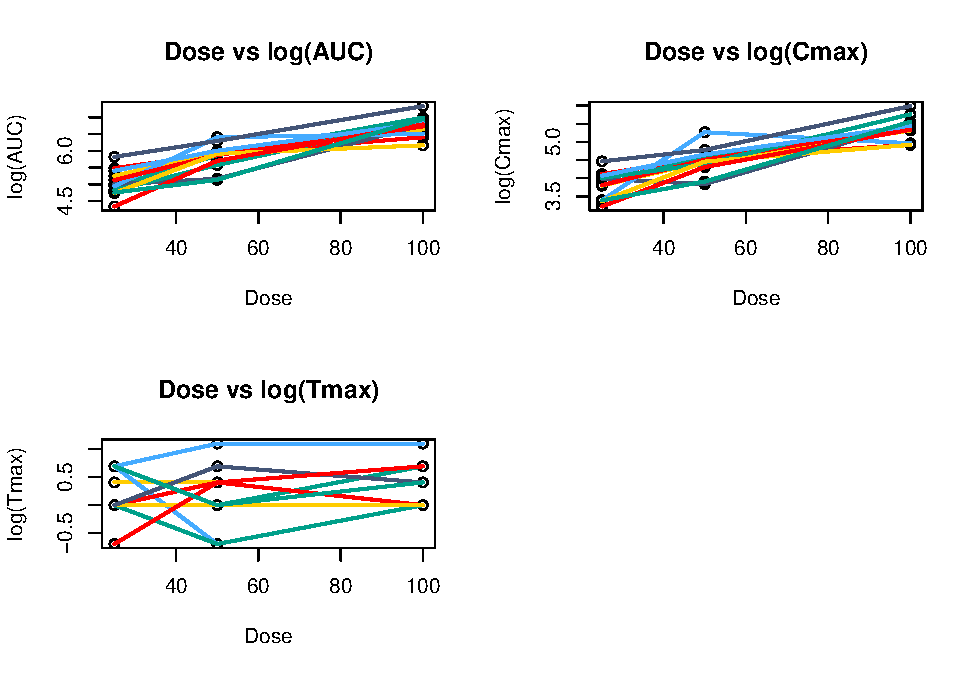
\includegraphics{perm_files/figure-latex/unnamed-chunk-41-1} \end{center}

Now the analysis: A simple solution could be:

\begin{Shaded}
\begin{Highlighting}[]
\FunctionTok{library}\NormalTok{(flip)}
\NormalTok{res}\OtherTok{=}\FunctionTok{flip}\NormalTok{(.}\SpecialCharTok{\textasciitilde{}}\NormalTok{Dose,}\AttributeTok{data=}\NormalTok{dati,}\AttributeTok{Strata=}\SpecialCharTok{\textasciitilde{}}\NormalTok{Sub,}\AttributeTok{statTest =} \StringTok{"coeff"}\NormalTok{)}
\FunctionTok{summary}\NormalTok{(res)}
\end{Highlighting}
\end{Shaded}

\begin{verbatim}
##  Call:
##  flip(Y = . ~ Dose, data = dati, statTest = "coeff", Strata = ~Sub) 
## 999 permutations.
## 
##       Test   Stat tail p-value sig.
## AUC  coeff 0.0221   ><  0.0010  ***
## Cmax coeff 0.0208   ><  0.0010  ***
## Tmax coeff 0.0024   ><  0.2680
\end{verbatim}

\begin{Shaded}
\begin{Highlighting}[]
\CommentTok{\#here we ask for statTest = "coeff", i.e. estimated coefficient of a linear model}
\FunctionTok{hist}\NormalTok{(res)}
\end{Highlighting}
\end{Shaded}

\begin{center}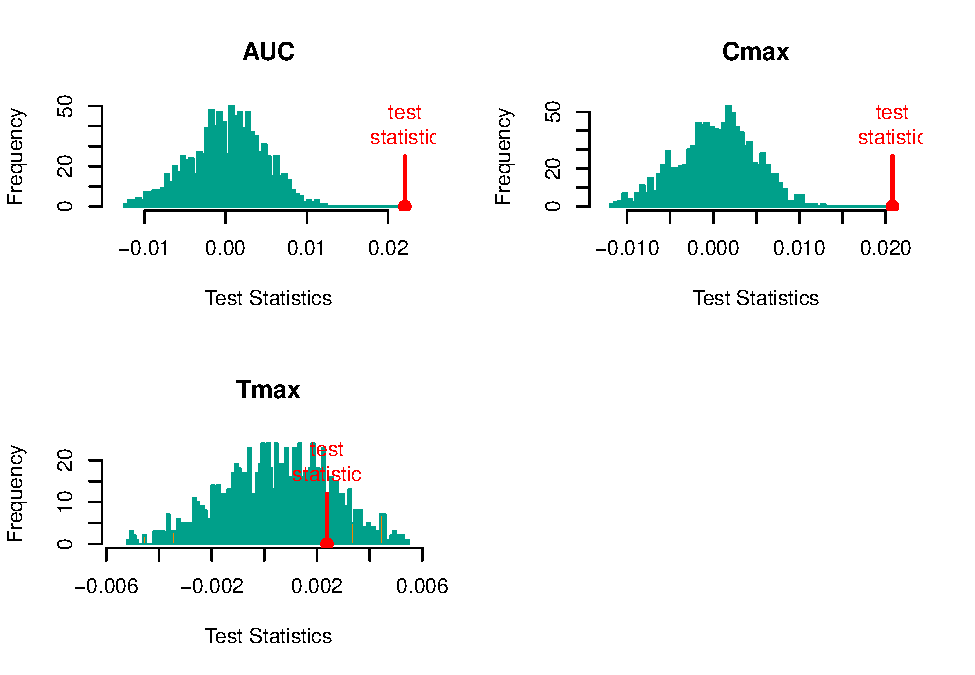
\includegraphics{perm_files/figure-latex/unnamed-chunk-42-1} \end{center}

Multivariate:

\begin{itemize}
\tightlist
\item
  Overall
\end{itemize}

\begin{Shaded}
\begin{Highlighting}[]
\NormalTok{res}\OtherTok{=}\FunctionTok{flip.adjust}\NormalTok{(res)}
\FunctionTok{npc}\NormalTok{(res,}\StringTok{"Fisher"}\NormalTok{)}
\end{Highlighting}
\end{Shaded}

\begin{verbatim}
## 
##    comb.funct nVar  Stat p-value
## V1     Fisher    3 15.13  0.0010
\end{verbatim}

There is an effect of \texttt{Dose}, overall.

\begin{itemize}
\tightlist
\item
  By end-points (closed testing with max-t combining function). Try also
  different methods (e.g.~\texttt{method="Fisher"}) and compare the
  results of \texttt{method="minP"} with the one of
  \texttt{method="Holm"}.
\end{itemize}

\begin{Shaded}
\begin{Highlighting}[]
\NormalTok{res}\OtherTok{=}\FunctionTok{flip.adjust}\NormalTok{(res,}\AttributeTok{method=}\StringTok{"holm"}\NormalTok{)}
\NormalTok{res}\OtherTok{=}\FunctionTok{flip.adjust}\NormalTok{(res,}\AttributeTok{method=}\StringTok{"Fisher"}\NormalTok{)}
\FunctionTok{summary}\NormalTok{(res)}
\end{Highlighting}
\end{Shaded}

\begin{verbatim}
##  Call:
##  flip(Y = . ~ Dose, data = dati, statTest = "coeff", Strata = ~Sub) 
## 999 permutations.
## 
##       Test   Stat tail p-value Adjust:maxT Adjust:holm Adjust:Fisher sig.
## AUC  coeff 0.0221   ><  0.0010      0.0010      0.0030        0.0030   **
## Cmax coeff 0.0208   ><  0.0010      0.0010      0.0030        0.0020   **
## Tmax coeff 0.0024   ><  0.2680      0.2680      0.2680        0.2680
\end{verbatim}

\texttt{AUC} and \texttt{Cmax} show a significant effect after
correction for multiplicity, while \texttt{Tmax} does not.

\hypertarget{minimal-bibliography}{%
\section{(minimal) Bibliography}\label{minimal-bibliography}}

The Grounding Theory:\\
- Pesarin (2001) Multivariate Permutation Tests: With Applications in
Biostatistics by Fortunato, Wiley, New York

An alternative approach to the Permutation testing:\\
- Hemerik J, Goeman J. Exact testing with random permutations. Test
(Madr). 2018;27(4):811-825. doi: 10.1007/s11749-017-0571-1. Epub 2017
Nov 30. PMID: 30930620; PMCID: PMC6405018.

A flexible approach to General Linear Model based on the sign-flip score
test:\\
- Hemerik, Goeman and Finos (2020) Robust testing in generalized linear
models by sign flipping score contributions. Journal of the Royal
Statistical Society Series B (Statistical Methodology) 82(3). DOI:
10.1111/rssb.12369\\
Implemented in R package flipscores:\\
\url{https://cran.r-project.org/web/packages/flipscores/index.html}~\\
better to use the github develop version:\\
\url{https://github.com/livioivil/flipscores}

A nice review of the regression model within the permutation
framework:\\
- Anderson M. Winkler, Gerard R. Ridgway, Matthew A. Webster, Stephen M.
Smith, Thomas E. Nichols (2014) Permutation inference for the general
linear model, NeuroImage, Volume 92, Pages 381-397, ISSN 1053-8119
\url{https://doi.org/10.1016/j.neuroimage.2014.01.060}

\end{document}
